\def\coursename{线性代数}
\def\coursefullname{线性代数}
\def\courseEnglishname{Linear Algebra}
\def\teachername{颜文斌}
\def\beginday{2021/12/28}

\documentclass[a4paper, 11pt]{article}

\usepackage[UTF8]{ctex}

\usepackage[T1]{fontenc}								% 字体
\catcode`\。=\active
\newcommand{。}{.} % {\ifmmode\text{.}\else .\fi}
\catcode`\(=\active
\catcode`\)=\active
\newcommand{(}{(}
\newcommand{)}{)}

% \usepackage{zhlineskip}

\usepackage{nicematrix}
% \usepackage{setspace}
% \linespread{1}						% 一倍行距
\setlength{\headheight}{14pt}			% 页眉高度
% \setlength{\lineskip}{0ex}			% 行距
\renewcommand\arraystretch{.82}		% 表格

\usepackage{amssymb, amsmath, amsfonts, amsthm}			% 数学符号,公式,字体,定理环境
\everymath{\displaystyle}			% \textstyle \scriptstyle \scriptscriptstyle
\allowdisplaybreaks[4]      		% 使用行间公式格式
% \makeatletter
% \renewcommand{\maketag@@@}[1]{\hbox{\m@th\normalsize\normalfont#1}}
% \makeatother
\newif\ifcontent\contenttrue		% if 显示目录
\newif\ifparskip\parskipfalse		% if 增加目录后的行距
\newif\ifshowemail\showemailfalse	% if 显示 email
\def\firstandforemost{
	\maketitle
	%\thispagestyle{empty}\clearpage
	\ifcontent
		\renewcommand{\contentsname}{目录}
		\tableofcontents
		\thispagestyle{empty}
		\clearpage
	\fi
	\ifparskip
		\setlength{\parskip}{.8ex}	% 设置额外的段距,目录后
	\fi								% 在 \firstandforemost 前设置 \parskiptrue
	\makenomenclature
	\printnomenclature
	\setcounter{page}{1}
}

\usepackage{mathtools}									% \rcase 环境等

% \usepackage{physics}

\usepackage[]{siunitx}									% 国际制单位
\sisetup{
	inter-unit-product = \ensuremath{{}\cdot{}},
	per-mode = symbol,
	per-mode = reciprocal-positive-first,
	range-units = single,
	separate-uncertainty = true,
	range-phrase = \ifmmode\text{\;-\;}\else\;-\;\fi
}
\DeclareSIUnit\angstrom{\text{Å}}
\DeclareSIUnit\atm{\text{atm}}
% SIunits 额外定义了一个 \square 表示平方,
% 还会把 \cdot 空格加大,真有够无语的 😅

\usepackage{authblk}									% 作者介绍
\ifx \coursefullname\undefined
	\ifx \coursename\undefined
		\def\coursename{笔记}
	\fi
	\def\coursefullname{\coursename}
\fi
\ifx \authorname\undefined
	\def\authorname{Dait}
\fi
\ifx \departmentname\undefined
	\def\departmentname{THU}
\fi
\ifx \emailaddress\undefined
	\def\emailaddress{daiyj20@mails.tsinghua.edu.cn}
\fi
\ifx \beginday\undefined
	\def\beginday{2021}
\fi
\ifx \endday\undefined
	\def\endday{\number\year/\number\month/\number\day}
\fi
\ifx \titleannotation\undefined
	\ifx \teachername\undefined
		\title{\textbf{\coursefullname}}
	\else
		\title{\textbf{\coursefullname}\\\small\textit{主要整理自\teachername 老师讲义}}
	\fi
\else
	\title{\textbf{\coursefullname}\\\small\textit{(\titleannotation)}}
\fi
\newif\ifdefaultauthor\defaultauthortrue
\ifdefaultauthor
	\author{by~\authorname~at~\departmentname}
	\ifshowemail
		\affil{\emailaddress}
	\fi
\fi
\ifx \endday\beginday
	\date{\beginday}
\else
	\date{\beginday~-~\endday}
\fi

\usepackage{hyperref}									% 链接
\ifx \courseEnglishname\undefined
	\def\courseEnglishname{Note}
\fi
\ifx \authorEnglishname\undefined
	\def\authorEnglishname{Dait}
\fi
\hypersetup{
	% dvipdfm								% 表示用 dvipdfm 生成 pdf
	pdftitle={\coursename},
	pdfauthor={\authorname},
	colorlinks=true, breaklinks=true,		% 超链接设置
	linkcolor=black, citecolor=black, urlcolor=blue
}

\usepackage[british]{babel}								% 长单词自动连字符换行
\hyphenation{long-sen-ten-ce}				% 自定义拆分方式

\usepackage{tikz}
\usetikzlibrary{quotes, angles}
\usepackage{pgfplots}
\pgfplotsset{compat=1.17}								% TikZ
\newcommand{\coor}[5][0]{
	\draw[thick,latex-latex](#1,#3)node[left]{$#5$}--(#1,0)node[shift={(-135:7pt)}]{$O$}--(#1+#2,0)node[right]{$#4$}
}			% 坐标轴

\usepackage{enumerate}									% 编号
\usepackage{paralist}
\setlength{\pltopsep}{1ex}
\setlength{\plitemsep}{1ex}
\ifx \eqnrange\undefined
	\numberwithin{equation}{section}
\else
	\numberwithin{equation}{\eqnrange}
\fi

\renewcommand{\thempfootnote}{\Roman{mpfootnote}}
\renewcommand{\thefootnote}{\Roman{footnote}}		% 注释上标 I, II,...
\newcommand{\sectionstar}[1]{
	\section[\hspace{-.8em}*\hspace{.3em}#1]{\hspace{-1em}*\hspace{.5em}#1}
}
\newcommand{\subsectionstar}[1]{					% 带星号的 section 和 subsection
	\subsection{\hspace{-1em}*\hspace{.5em}#1}
}
\newcommand{\subsubsectionstar}[1]{					% 带星号的 section 和 subsection
	\subsubsection{\hspace{-1em}*\hspace{.5em}#1}
}
\newcommand*{\appendiks}{
	\appendix
	\part*{附录}
	\addcontentsline{toc}{part}{附录}
}
\iffalse			% 不清楚
	\newcommand{\varsection}[1]{
		\refstepcounter{section}
		\section*{\thesection\quad #1}
		\addcontentsline{toc}{section}{\makebox[0pt][r]{*}\thesection\quad #1}
	}
\fi

\usepackage{fancyhdr}									% 页眉页脚
\ifx \coursename\undefined
	\def\coursename{笔记}
\fi
\fancyhf{}\pagestyle{fancy}
\fancyhead[L]{\coursename\rightmark}
\fancyhead[R]{by~\authorname}
\fancyfoot[C]{-~\thepage~-} 			%页码

\usepackage{colortbl, booktabs}							% 表

\usepackage{graphicx}
\usepackage{float}
\usepackage{caption}									% 图
\captionsetup{
	margin=20pt, format=hang,
	justification=justified
}
\newcounter{tikzpic}
\def\tikzchap{
	\stepcounter{tikzpic}\\
	\small 图~\thetikzpic\quad
}
\newcounter{linetable}
\newcommand{\tablechap}[1]{
	\stepcounter{linetable}
	{\small 表~\thelinetable\quad #1}\\[1em]
}

\usepackage{tcolorbox}									% 盒子
\tcbuselibrary{theorems, skins, breakable}
\definecolor{MatchaGreen}{HTML}{73C088}		% 抹茶绿B7C6B3
\newtcbtheorem[number within = subsection]{example}{例}{
	enhanced, breakable, sharp corners,
	attach boxed title to top left = {yshifttext = -1mm},
	before skip = 2ex,
	colback = MatchaGreen!5,				% 文本框内的底色
	colframe = MatchaGreen,					% 文本框框沿的颜色
	fonttitle = \bfseries,					% 标题字体用粗体	coltitle 默认 white,
	boxed title style = {
			sharp corners, size = small, colback = MatchaGreen,
		}
}{exm}
\definecolor{MelancholyBlue}{HTML}{9EAABA}	% melancholy: 沮丧
\newcounter{pslt}
\setcounter{pslt}{-1}
\newtcbtheorem[use counter = pslt]{posulate}{假设}{
	enhanced, breakable, sharp corners,
	attach boxed title to top left = {yshifttext = -1mm}, before skip = 2ex,
	colback = MelancholyBlue!5, colframe = MelancholyBlue, fonttitle = \bfseries,
	boxed title style = {
			sharp corners, size = small, colback = MelancholyBlue,
		}
}{psl}
\definecolor{PureBlue}{HTML}{80A3D0}
\newtcbtheorem[number within = subsection]{definition}{定义}{
	enhanced, breakable, sharp corners,
	attach boxed title to top left = {yshifttext = -1mm}, before skip = 2ex,
	colback = PureBlue!5, colframe = PureBlue, fonttitle = \bfseries,
	boxed title style = {
			sharp corners, size = small, colback = PureBlue,
		}
}{dfn}
\definecolor{PeachRed}{HTML}{EA868F}
\newtcbtheorem[number within = subsection]{theorem}{定理}{
	enhanced, breakable, sharp corners,
	attach boxed title to top left = {yshifttext = -1mm}, before skip = 2ex,
	colback = PeachRed!5, colframe = PeachRed, fonttitle = \bfseries,
	boxed title style = {
			sharp corners, size = small, colback = PeachRed,
		}
}{thm}
\definecolor{SchembriumYellow}{HTML}{fbd26a}	% 申博太阳城黄
\newtcbtheorem[number within = section]{method}{方法}{
	enhanced, breakable, sharp corners,
	attach boxed title to top left = {yshifttext = -1mm}, before skip = 2ex,
	colback = SchembriumYellow!5, colframe = SchembriumYellow, fonttitle = \bfseries,
	boxed title style = {
			sharp corners, size = small, colback = SchembriumYellow,
		}
}{mtd}
% 保留颜色
\definecolor{fadedgold}{HTML}{D9CBB0}		% 褪色金
\definecolor{saturatedgold}{HTML}{F0E0C2}	% staurated: 饱和
\definecolor{elegantblue}{HTML}{C4CCD7}		% elegant: 优雅
\definecolor{ivory}{HTML}{F1ECE6}			% 象牙
\definecolor{gloomypruple}{HTML}{CCC1D2}	% 阴沉紫
% \textcolor[HTML]{FFC23A}					% 石板灰

\definecolor{Green}{rgb}{0,.8,0}

\usepackage{imakeidx}								% 索引

\usepackage{nomencl}								% 关键词
%\setlength{\nomitemsep}{0.2cm}							% 设置术语之间的间距
\renewcommand{\nomentryend}{.}							% 设置打印出术语的结尾的字符
\renewcommand{\eqdeclaration}[1]{见公式:(#1)}			% 设置打印见公式的样式
\renewcommand{\pagedeclaration}[1]{见第 (#1) 页}		% 设置打印页的样式
\renewcommand{\nomname}{术语表} 						% 修改术语表标题的名称。

\usepackage{array}
\usepackage{booktabs} % 三线表
\usepackage{multirow}
% 手动排版,尽量杜绝使用

\newcommand{\bs}[1]{\hspace{-#1 pt}}		% 手动减间距	backspace
\newcommand{\bv}[1]{\vspace{-#1 pt}}		% 手动缩行距	backvspace
\def\directlisteqn{\vspace{-1ex}}
\iffalse									% 尽量避免孤行
	\widowpenalty=4000
	\clubpenalty=4000
\fi

% 杂项符号
\def\avg{\overline}
\newcommand*{\rqed}{\tag*{$\square$}}								% 靠右 QED
\newcommand*{\halfqed}{\tag*{$\boxdot$}}
\newcommand*{\thus}{\quad\Rightarrow\quad}							% =>
\newcommand*{\ifnf}{\quad\Leftrightarrow\quad}						% <=>	if and only if
\newcommand*{\turnto}{\quad\to\quad}
\newcommand*{\normalize}{\quad\overset{\mathrm{normalize}}{-\!\!\!-\!\!\!-\!-\!\!\!\longrightarrow}\quad}
\newcommand*{\vthus}{\\$\Downarrow$\\}
\newcommand*{\viff}{\\$\Updownarrow$\\}
\newcommand*{\vs}{~\text{-}~}
\newcommand{\eg}[1][]{\subparagraph*{例#1:}}
\newcommand*{\prf}{\noindent\textbf{证明:}\quad}
\newcommand{\dpfr}[2]{\displaystyle\frac{#1}{#2}}					% 大分数
\newcommand{\frdp}[2]{\frac{\displaystyle #1}{\displaystyle #2}}
\newcommand{\spark}[1]{\;\textcolor{red}{#1}}

% 简化更常用的希腊字母
\newcommand*{\vf}{\varphi}
\newcommand*{\vF}{\varPhi}
\newcommand*{\vp}{\varPsi}
\newcommand*{\ve}{\varepsilon}
\newcommand*{\vC}{\varTheta}
\newcommand*{\ct}{\theta}			% 还是建议用 @ + Tab 快捷键

% 正体符号
\newcommand*{\cns}{\mathrm{const}}
\newcommand*{\plusc}{{\color{lightgray}\,+\,\cns}}
\newcommand*{\e}{\mathop{}\!\mathrm{e}^}	% e
\let\accenti\i
\renewcommand*{\i}{\mathrm{i}}
\newcommand*{\D}{\Delta}
\newcommand*{\p}{\partial}

\usepackage{bm}											% 粗体 \bm
\newcommand{\hbm}[1][r]{\hat{\bm #1}}	% 应该不会有两个字母的
\newcommand{\ibm}[1]{\,\bm #1}

% Using EnglischeSchT script font style
\newfontfamily{\calti}{EnglischeSchT}
\newcommand{\mathcalti}[1]{\mbox{\calti{#1}}}
\newcommand{\mathcaltibf}[1]{\mbox{\bf\calti{#1}}}

\usepackage{mathrsfs}									% 花体 \mathscr
% \usepackage{boondox-cal}								% 小写花体 \mathcal
\newcommand*{\RR}{\mathbb R}
\newcommand*{\CC}{\mathbb C}
\newcommand*{\ZZ}{\mathbb Z}
\newcommand*{\sC}{\mathscr C}			% n 阶连续可导函数
\newcommand*{\sR}{\mathscr R}			% 黎曼可积
% 算符用 \mathcal
\newcommand*{\cL}{\mathcal L}			% 表示一般算子
\newcommand{\cl}[1]{\mathcal L\fkh{#1}}
\newcommand{\cli}[1]{\mathcal L^{-1}\!\fkh{#1}}
\newcommand{\cf}[2][\!\,]{\mathcal F_\mathrm{#1}\fkh{#2}}
\newcommand{\cfi}[2][\!\,]{\mathcal F_\mathrm{#1}^{-1}\!\fkh{#2}}
% \newcommand{\cl}[2][0]{\mathcal L\ikh[#1]{#2}}
% \newcommand{\cli}[2][0]{\mathcal L^{-1}\ikh[#1]{#2}}
% \newcommand{\cf}[2][0]{\mathcal F\ikh[#1]{#2}}
% \newcommand{\cfi}[2][0]{\mathcal F^{-1}\ikh[#1]{#2}}

\usepackage{cancel}										% 删除线

\usepackage{xfrac}

% \usepackage{emoji}	需要 LuaTeX

% 导数等
\let\divides\div
\renewcommand*{\div}{\nabla\cdot}
\newcommand*{\curl}{\nabla\times}
\newcommand*{\lap}{\Delta}
\let\accentd\d
\renewcommand*{\d}{\mathop{}\!\mathrm{d}}
\newcommand*{\nd}{\mathrm{d}}
\newcommand*{\vd}{\mathop{}\!\delta}											% δ
\newcommand{\dd}[2][\;\!\!]{\frac{\nd^{#1}}{\nd #2^{#1}}}						% d/dx			我知道 \,\! 很愚蠢,但是 {} 无法在 Math Preview 上预览
\newcommand{\dn}[2]{\frac{\nd^{#1}}{\nd #2^{#1}}}								% d^n/dx^n		\dn2x≡\dd[2]x
\newcommand{\dv}[3][\;\!\!]{\frac{\nd^{#1}#2}{\nd #3^{#1}}}						% df/dx
\newcommand{\du}[3]{\frac{\nd^{#1}#2}{\nd #3^{#1}}}								% d^nf/dx^n		\du2fx≡\dv[2]fx
\newcommand{\pp}[2][\;\!\!]{\frac{\p^{#1}}{\p #2^{#1}}}							% ∂/∂x
\newcommand{\pn}[2]{\frac{\p^{#1}}{\p #2^{#1}}}									% ∂^n/∂x^n		\pn2x≡\pp[2]x
\newcommand{\pv}[3][\;\!\!]{\frac{\p^{#1}#2}{\p #3^{#1}}}						% ∂f/∂x
\newcommand{\pu}[3]{\frac{\p^{#1}#2}{\p #3^{#1}}}								% ∂^nf/∂x^n		\pu2x≡\pv[2]x
\newcommand{\pw}[3]{\frac{\p^2 #1}{\p #2\p #3}}									% ∂^2f/∂x∂y
\newcommand{\pvv}[6]{															% ∂^(m+n)f/∂x^m∂y^n
	\ifnum#4=1
		\ifnum#6=1
			\frac{\p^{#1}#2}{\p #3\p #5}
		\else
			\frac{\p^{#1}#2}{\p #3\p #5^{#6}}
		\fi
	\else
		\ifnum#6=1
			\frac{\p^{#1}#2}{\p #3^{#4}\p #5}
		\else
			\frac{\p^{#1}#2}{\p #3^{#4}\p #5^{#6}}
		\fi
	\fi}
\newcommand{\dvd}[2]{\left.#1\middle\slash #2\right.}							% 斜除

% 积分
\newcommand*{\intt}{\bs2\int\bs8\int}											% ∫∫
\newcommand*{\inttt}{\int\bs8\int\bs8\int}										% ∫∫∫
\newcommand*{\intdt}{\int\bs3\cdot\bs2\cdot\bs2\cdot\bs4\int}					% ∫...∫
\newcommand*{\zti}{_0^{+\infty}}												% _0^+∞
\newcommand*{\iti}{_{-\infty}^{+\infty}}										% _-∞^+∞
\newcommand{\fmto}[3][\infty]{_{#2=#3}^{#1}}

% 括号
\newcommand{\abs}[1]{\left\lvert#1\right\rvert}									% |x| 绝对值
\newcommand{\norm}[1]{\left\lVert#1\right\rVert}								% ||x|| 模
\newcommand{\edg}[1]{\left.#1\right\rvert}										% f|  竖线
\newcommand{\kh}[1]{\left(#1\right)}											% (x) 括号
\newcommand{\fkh}[1]{\left[#1\right]}											% [x] 方括号
\newcommand{\hkh}[1]{\left\{#1\right\}}											% {x} 花括号
\newcommand{\zkh}[1]{\lfloor\bs{4.7}\lceil #1\rceil\bs{4.7}\rfloor}				% [x] 中括号
\newcommand{\ikh}[2][0]{\ifnum#1=0 \zkh{#2}\else \fkh{#2}\fi}					% [x] 可调大小的中括号
\newcommand{\set}[2]{\left\{#1\,\middle\vert\,#2\right\}}						% {x|x1,x2,...} 集合
\newcommand{\ave}[1]{\left\langle #1\right\rangle}								% <x> 平均值
\newcommand{\bra}[1]{\left\langle #1\right\vert}								% <ψ| 左矢
\newcommand{\ket}[1]{\left\vert #1\right\rangle}								% |ψ> 右矢
\newcommand{\brkt}[2]{\left\langle #1\middle\vert #2\right\rangle}				% <φ|ψ> 内积
\newcommand{\ktbr}[2]{\left\vert#1\right\rangle \bs3\left\langle #2\right\vert}	% |ψ><φ|
\newcommand{\inp}[2]{\left\langle #1,#2\right\rangle}							% <f,g> 内积

% 数学运算符
\let\Real\Re
\let\Imagin\Im
\let\Re\relax
\let\Im\relax
\DeclareMathOperator{\Re}{Re}					% 
\DeclareMathOperator{\Im}{Im}					% 
\DeclareMathOperator{\sech}{sech}				% 
\DeclareMathOperator{\csch}{csch}				% 
\DeclareMathOperator{\arcsec}{arcsec}			% 
\DeclareMathOperator{\arccot}{arccot}			% 
\DeclareMathOperator{\arccsc}{arccsc}			% 
\DeclareMathOperator{\arsinh}{arsinh}			% 
\DeclareMathOperator{\arcosh}{arcosh}			% 
\DeclareMathOperator{\artanh}{artanh}			% 
\DeclareMathOperator{\sgn}{sgn}					% 符号函数
\DeclareMathOperator{\Li}{Li}					% 
\DeclareMathOperator{\Si}{Si}
\DeclareMathOperator{\Ci}{Ci}
\DeclareMathOperator{\sinc}{sinc}
\DeclareMathOperator{\Heaviside}{H}
\DeclareMathOperator{\arr}{A}					% 排列数
\DeclareMathOperator{\com}{C}					% 组合数
\DeclareMathOperator{\Res}{Res}					% 留数
\DeclareMathOperator{\supp}{supp}
\newcommand*{\bigo}{\mathcal O}

% 线性代数
\newif\ifLinearAlgebra\LinearAlgebratrue
\ifLinearAlgebra
\DeclareMathOperator{\rank}{rank}
\DeclareMathOperator{\id}{id}
\newcommand*{\tp}{^{\mathrm T}}				% AT 转置
\newcommand*{\cj}{^\ast}					% A* 共轭
\newcommand*{\dg}{^\dagger}					% A† 共轭转置
\newcommand*{\iv}{^{-1}}					% A-1
\fi

% 物理学家
\newcommand*{\Schr}{Schrödinger}
\newcommand*{\Legd}{Legendre}
\newcommand*{\deB}{de Broglie}
\newcommand*{\Rayl}{Rayleigh}
\newcommand*{\Lande}{Landé}

% 粒子
\newcommand*{\elc}{\mathrm e}
\newcommand*{\pton}{\mathrm p}
\newcommand*{\mol}{\mathrm m}

% 物理常数
\newcommand*{\NA}{N_{\bs1\mathrm A}}						% Avogadro 常数
\newcommand*{\kB}{k_{\mathrm B}}							% Boltzmann 常数
\newcommand*{\muB}{\mu_\mathrm B}							% Bohr 磁矩

% 
\newcommand*{\Ek}{E_{\mathrm k}}							% 动能
\newcommand*{\eff}{_\mathrm{eff}}							% 有效下标
\newcommand*{\tot}{_\mathrm{tot}}
\newcommand*{\lSI}{\tag{SI}}
\newcommand*{\CGS}{\tag{CGS}}								% cm, g, s 制


\newcommand*{\FF}{\mathbb F}
\newcommand*{\PP}{\mathbb P}
\newcommand*{\Lm}{\varLambda}
\DeclareMathOperator{\row}{row}
\DeclareMathOperator{\col}{col}
\let\oldC\C
\let\C\relax
\DeclareMathOperator{\C}{C}
\DeclareMathOperator{\N}{N}
\DeclareMathOperator{\rem}{ref}
\DeclareMathOperator{\rrem}{rref}
\DeclareMathOperator{\spn}{span}
\DeclareMathOperator{\diag}{diag}
\DeclareMathOperator{\adj}{adj}
\DeclareMathOperator{\tr}{tr}
\DeclareMathOperator{\ord}{ord}
\DeclareMathOperator{\sym}{sym}
\DeclareMathOperator{\GL}{GL}		% general linear

\begin{document}
\firstandforemost

\section{向量和矩阵}
\subsection{向量}
\begin{definition}{向量}{vector}
	在数域(number field)~$\FF$\footnote{直到第~\ref{sec:complex linear space}~章复线性空间之前,均只考虑实数域$\RR$,即$\FF=\RR$。}~内,一个$n$维向量(vector)~$v$由$n$个标量(scalar)~$v_1,\ldots,v_n$组成,记作
	\[
		v=\begin{bmatrix}
			v_1\\\vdots\\v_n
		\end{bmatrix},\quad v_i\in\FF.
	\]
	组成向量的标量$v_1,\ldots,v_n$称为向量的分量(component)。
	%向量的维度$\dim(v)=n$即分量的个数。
\end{definition}
\begin{definition}{零向量、反向量}{zero vector}
	零向量(zero vector)是所有分量均为0的向量,记作0;
	
	$v$的反向量(reverse vector)对应每个分量取相反数,记作$-v$。
\end{definition}
\begin{definition}{向量的加法}{vector addition}
	向量的加法(addition)即对应分量相加,
	\[
		v+u=\begin{bmatrix}
			v_1\\\vdots\\v_n
		\end{bmatrix}+\begin{bmatrix}
			u_1\\\vdots\\u_n
		\end{bmatrix}=\begin{bmatrix}
			v_1+u_1\\\vdots\\v_n+u_n
		\end{bmatrix}.
	\]
	因此只有分量数相同的向量之间才可以相加。
\end{definition}
\begin{compactitem}
	\item 交换律:$v+u=u+v;$
	\item 结合律:$v+(u+w)=(v+u)+w.$
	\item 零向量:$0+v=v+0=v.$
	\item 反向量:$v+(-v)=0.$
\end{compactitem}
\begin{definition}{向量的数乘}{vector scalar product}
	向量与标量的数乘(scalar product)即每个分量乘标量
	\[
		cv=c\begin{bmatrix}
			v_1\\\vdots\\v_n
		\end{bmatrix}=\begin{bmatrix}
			cv_1\\\vdots\\cv_n
		\end{bmatrix}.
	\]
\end{definition}
\begin{compactitem}
	\item $1v=v,\;(-1)v=-v,\;0v=0.$
	\item 结合律:$c(dv)=(cd)v\equiv cdv;$
	\item 对标量的分配律:$(c+d)v=cv+dv;$
	\item 对向量的分配律:$c(v+u)=cv+cu.$
\end{compactitem}
\begin{definition}{线性组合}{linear combination}
	向量$v$和$u$的线性组合(linear combination)定义为
	\[
		cv+du,\quad c,d\in\FF.
	\]
	以此类推,$n$个向量$v_1,v_2,\ldots,v_n$的线性组合形如
	\[
		c_1v_1+c_2v_2+\cdots+c_nv_n,\quad c_i\in\FF.
	\]
\end{definition}
\begin{definition}{向量的内积}{vector inner product}
	向量$v$和$u$的内积(inner product)结果是一个标量,其值为
	\begin{equation}
		v\cdot u:=\sum_{i=1}^nv_iu_i=v_1u_1+v_2u_2+\cdots+v_nu_n.
	\end{equation}
	特别的,$v^2:=v\cdot v.$
\end{definition}
\begin{compactitem}
	\item 交换律:$v\cdot u=u\cdot v;$
	\item 与数乘的结合律:$(cv)\cdot u=c(v\cdot u)\equiv cv\cdot u;$
	\item 分配律:$(v+u)\cdot w=v\cdot w+u\cdot w;$
	\item $v^2\geqslant 0$,取等号当且仅当$v=0.$
\end{compactitem}
\begin{definition}{向量的长度}{vector norm}
	通过内积我们可以定义向量的长度(norm)
	\begin{equation}
		\norm v:=\sqrt{v^2}=\kh{v_1^2+v_2^2+\cdots+v_n^2}^{1/2}.
	\end{equation}
	单位向量(unit vector)就是长度为1的向量。
\end{definition}
显然,和$v$同向的单位向量是$\hat v:=v/\norm v.$
\iffalse
\begin{definition}{两向量间的夹角}{angle between two vectors}
	定义向量的夹角$\theta\in[0,\pi]$满足
	\[
		\cos\theta=\frac{v\cdot u}{\norm v\norm u}.
	\]
\end{definition}
%故$v\perp u\ifnf v\cdot u=0$。
\begin{theorem}{Cauchy不等式}{Cauchy Inequality}
	因为$\abs{\cos\theta}\leqslant 1$,故 
	\begin{equation}
		\abs{v\cdot u}\leqslant\norm v\norm u.
	\end{equation}
\end{theorem}
\fi
\subsection{矩阵}
形式上看,标量$c$是$1\times 1$的,向量$v$是$m\times 1$的\footnote{如无特别说明,向量均默认为列向量。},继而可定义$m\times n$的矩阵(matrix)形如
\[
	A=\begin{bmatrix}
		A_{11}&\cdots&A_{1n}\\
		\vdots&\ddots&\vdots\\
		A_{m1}&\cdots&A_{mn}
	\end{bmatrix},\quad A_{ij}\in\FF.
\]
$A_{ij}$是矩阵第$i$行第$j$列的元素。

矩阵的行数和列数分别为$\row(A)=m$,$\col(A)=n$。当$m=n$时,矩阵是$n$阶方阵(square matrix)。

矩阵的加法和数乘与向量的运算规律相同,是平凡的。
\begin{definition}{矩阵和向量的乘法}{Matrix Vector Product}
	$m\times n$矩阵$A$乘$n$维向量$x$,结果是一个$m$维向量$b=Ax$,其分量为:
	\begin{equation}
		b_i=\sum_{j=1}^nA_{ij}x_j,\quad i=1,\ldots,m.
	\end{equation}
\end{definition}
因此$Ax$是看成$A$所有列的线性组合,或者说$A$的各行与$x$分别内积。这样线性方程组就可以写成矩阵的形式:
\[
	Ax=b.
\]
这种思想有助于我们掌握线性代数的理念。
\begin{definition}{矩阵的乘法}{Matrix Product}
	$m\times n$矩阵$A$乘$n\times p$矩阵$B$,结果是一个$m\times p$的矩阵$C=AB$,其分量为
	\begin{align}
		C_{ij}=\sum_{k=1}^nA_{ik}B_{kj}.
	\end{align}
	因此若$A,B$可以相乘,要求$\col(A)=\row(B).$
\end{definition}
\begin{compactitem}
	\item 一般不满足交换律,即$AB\neq BA$,比如
	\[
		\begin{bmatrix}
			0&1\\1&0
		\end{bmatrix}\begin{bmatrix}
			1&0\\0&-1
		\end{bmatrix}=\begin{bmatrix}
			0&-1\\1&0
		\end{bmatrix},\quad\begin{bmatrix}
			1&0\\0&-1
		\end{bmatrix}\begin{bmatrix}
			0&1\\1&0
		\end{bmatrix}=\begin{bmatrix}
			0&1\\-1&0
		\end{bmatrix}.
	\]
	\item 左分配律:$(A+B)C=AC+BC;$
	\item 右分配律:$A(B+C)=AB+AC.$
\end{compactitem}
\begin{theorem}{矩阵乘法的结合律}{associative law of matrix multiplication}
	\begin{equation}
		(AB)C=A(BC)\equiv ABC.
	\end{equation}
\end{theorem}
\prf 对于$A_{m\times n},B_{n\times p},C_{p\times q}$
\begin{align*}
	\bigfkh{A(BC)}_{ij}&=\sum_{k=1}^nA_{ik}(BC)_{kj}=\sum_{k=1}^nA_{ik}\sum_{\ell=1}^pB_{k\ell}C_{\ell j}\\
	&=\sum_{\ell=1}^p\sum_{k=1}^nA_{ik}B_{k\ell}C_{\ell j}=\sum_{\ell=1}^p(AB)_{i\ell}C_{\ell j}=\bigfkh{(AB)C}_{ij}.\rqed
\end{align*}
\begin{definition}{单位矩阵}{unit matrix}
	$n$阶单位矩阵(unit matrix)是$n$阶方阵,对角项均为1,其余项均为0:
	\[
		I_n=\begin{bmatrix}
		1&\\ &\ddots\\&&1
		\end{bmatrix}.
	\]
\end{definition}
易证,$\forall m\times n$的矩阵$A$,均有
\[
	I_mA=AI_n=A.
\]
\begin{theorem}{交换性}{commutable}
	若方阵$A$与任意方阵可交换(commutable),则$A=cI,\;c\in\FF$
\end{theorem}
\prf 取$B=e_{ij}$,表示仅$i$行$j$列为1,其余项均为0
\begin{align*}
	(Ae_{ij})_{k\ell}=\sum_{p=1}^nA_{kp}(e_{ij})_{p\ell}=A_{ki}\delta_{j\ell};\\
	(e_{ij}A)_{k\ell}=\sum_{p=1}^n(e_{ij})_{kp}A_{p\ell}=\delta_{ki}A_{j\ell},
\end{align*}
当$k\neq i=j=\ell$时,$A_{ki}=0$;当$k=i\neq j=\ell$时,$A_{ii}=A_{jj}$。\qed
\begin{definition}{分块矩阵}{block matrix}
	可以将矩阵分块,每一块(block)是一个小矩阵,比如
	\begin{align*}
		\fkh{\begin{array}{cc|cc}
			1&0&1&0\\
			0&1&0&1\\
			\hline
			1&0&1&0\\
			0&1&0&1	
		\end{array}}\equiv\begin{bmatrix}
			I&I\\I&I
		\end{bmatrix}.
	\end{align*}
\end{definition}
分块矩阵乘法:每个块当作矩阵的元素,块之间使用矩阵乘法。
\subsection{矩阵的逆和转置}
\begin{definition}{矩阵的逆}{inverse matrix}
	方阵$A$的逆矩阵(inverse matrix)~$A\iv$满足
	\[
		AA\iv=A\iv A=I.
	\]
	称奇异矩阵(singular matrix)是不可逆的矩阵。
\end{definition}
若$A,B$均可逆,则$(AB)\iv=B\iv A\iv$。但$A+B$不一定可逆。
\begin{example}{二阶方阵的逆}{inverse of 2x2 matrix}
	\begin{equation}
		\begin{bmatrix}
			a&b\\c&d
		\end{bmatrix}\iv=\frac1{ad-bc}
		\begin{bmatrix}
			d&-b\\
			-c&a
		\end{bmatrix}.
	\end{equation}
\end{example}
\begin{example}{对角矩阵的逆}{inverse of diagonal matrix}
	非对角项均为0的方阵称为对角矩阵(diagonal matrix),若对角项为$a_1,\ldots,a_n$,可记作
	\[
		\diag(a_1,\ldots,a_n).
	\]
	对角矩阵有很多简单的性质,比如对角矩阵的乘法很简单
	\begin{align}
		\diag(a_1,\ldots,a_n)\diag(b_1,\ldots,b_n)=\diag(a_1b_1,\ldots,a_nb_n).
	\end{align}
	%故
	显然,对角矩阵的逆为
	\begin{align}
		\diag(a_1,\ldots,a_n)\iv=\diag(a_1^{-1},\ldots,a_n^{-1}).
	\end{align}
\end{example}
% 若$A$可逆,则方程组$Ax=b$的解为 \[x=A\iv b.\]
\begin{theorem}{左逆和右逆}{linverse and rinverse}
	%左逆等于右逆。
	%\prf 设方程$A$的左逆为$B$,右逆为$C$,即$BA=AC=I$,则 
	%\[B=B(AC)=(BA)C=C.\rqed\]
	%\tcblower
	若存在左逆(left inverse),则其也是右逆(right inverse)。
\end{theorem}
\prf 设$B$是$A$的左逆,即$BA=I$。构造映射$f,g$
\[
	f(X):=AXB,\quad g(X):=BXA,
\]
则$g\circ f(X)=BAXBA=X$,$g$是双射。又
\[
	g(AB)=BABA=I=g(I),
\]
故$AB=I$。\qed
\begin{example}{幂零矩阵}{nilpotent matrix}
	若$A$是幂零矩阵(nilpotent matrix),即$\exists n\in\mathbb N$使$A^n=O$,
	
	则$I+A$可逆,且
	\[
		(I+A)\iv=I-A+A^2-\cdots+(-A)^{n-1}.
	\]
	因为
	\[
		I=I^n+A^n=(I+A)\bigfkh{I^{n-1}-I^{n-2}A+\cdots+(-A)^{n-1}}.\rqed
	\]
\end{example}
%\subsection{矩阵的转置}
\begin{definition}{矩阵的转置}{transpose matrix}
	$m\times n$矩阵$A$的转置(transpose)~$A\tp$是$n\times m$矩阵,且 
	\[
		(A\tp)_{ij}=A_{ji}.
	\]
	特别的,若$S\tp=S$,则$S$是对称矩阵(sysmmetric matrix)。
\end{definition}
\begin{compactitem}
	\item $(A+B)\tp=A\tp+B\tp,\enspace (cA)\tp=cA\tp;$
	\item $(AB)\tp=B\tp A\tp;$
	\item $(A\iv)\tp=(A\tp)\iv.$
\end{compactitem}
\subsection{矩阵的迹}
\begin{definition}{矩阵的迹}{trace}
	$n$阶方阵的迹(trace)是对角元的和
	\begin{equation}
		\tr(A):=\sum_{i=1}^nA_{ii}.
	\end{equation}
\end{definition}
\begin{compactitem}
	\item $\tr(A+B)=\tr(A)+\tr(B),\enspace \tr(cA)=c\tr(A);$
	\item $\tr(A\tp)=\tr(A);$
	\item 两个$n$维列向量$u,v$,有$\tr(uv\tp)=v\tp u$
	\[
		\tr(uv\tp)=\sum_{i=1}^nu_iv_i=u\tp v=v\tp u.
	\]
	\item $\tr(AB)\neq\tr(A)\tr(B).$
\end{compactitem}
\begin{theorem}{交换矩阵乘法的迹}{trace of commute multiplication}
	$\forall m\times n$的矩阵$A$和$n\times m$的矩阵$B$,都有
	\begin{equation}
		\tr(AB)=\tr(BA).
	\end{equation}
\end{theorem}
\prf 
\begin{align*}
	\tr(AB)&=\sum_{i=1}^m(AB)_{ii}=\sum_{i=1}^m\sum_{j=1}^nA_{ij}B_{ji}\\
	&=\sum_{j=1}^n\sum_{i=1}^mB_{ji}A_{ij}=\sum_{j=1}^n(BA)_{jj}=\tr(BA).\rqed
\end{align*}
除此之外,迹还有一些重要性质,将在后面讲。
\clearpage
\section{线性方程组}
线性方程(linear equation)是未知数最高次数为1的方程。考虑$m$个$n$元线性方程构成的线性方程组(linear equation set)
\[
	\sum_{j=1}^nA_{ij}x_j=b_i.\quad i=1,2,\ldots,m.
\]
可以把系数写成系数矩阵$A$,即$Ax=b.$
\subsection{消元法}
\begin{definition}{消元法}{elimination}
	消元法(elimination)就是通过对方程之间倍加消元,得到一个上三角方程组,比如
	\[
		\begin{equationset}
			x-2y&=1\\3x+2y&=11
		\end{equationset}\thus
		\begin{equationset}
			x-2y&=1\\8y&=8
		\end{equationset}
	\]
	而主元(pivot element)就是每个方程第一个非0系数。
\end{definition}

消元法失效:主元数目$<$未知数
\begin{compactitem}
	\item 得到$0\neq 0$,无解;
	\item 得到$0=0$,无穷多解。
\end{compactitem}
因此消元法要求方程个数与未知数个数相同。

\begin{method}{消元法算法}{elimination algorithm}
	\begin{compactenum}
		\item 找到第1个$x_1$系数不为0的方程并移到最上面。%$x_1$的系数就是第一个主元。
		\item 从第2个到第$n$个方程中消去$x_1$ (方程$i-\ell_{i1}\times$\!\,方程1)。
		\item 得到第2个到第$n$个方程构成$(n-1)$元的线性方程组,重复步骤1。
		\item 最后结果要么是一个上三角方程组,要么失效。
		\item 上三角的情况,从最后一个方程开始解出全部未知数。
	\end{compactenum}
\end{method}

利用消元法,可以求矩阵的逆。
\begin{method}{Gauss-Jordan消元法}{Gauss-Jordan elimination}
	对增广矩阵(augmented matrix)\;$(A,I)$做消元操作。
	\[
		(A,I)\turnto(I,A\iv).
	\]
	就可以得到$A$的逆$A\iv$。
\end{method}
\subsection{矩阵的行变换}
方程中,置换、倍加、倍乘同时作用在系数矩阵$A$和$b$上,因此可以写成增广矩阵$(A,b)$并对其消元。类似的,可以考虑对一般矩阵进行置换、倍加、倍乘的操作。
\begin{definition}{矩阵的初等行变换}{}
	\begin{compactitem}
		\item 对换:交换两行
		\item 倍加:一行乘系数加到另一行
		\item 倍乘:一行乘以一个非零系数
	\end{compactitem}
\end{definition}
如果一个矩阵可以行变换成另一个矩阵,则它们行等价(equivalence)。

\begin{definition}{行阶梯矩阵}{row echelon matrix}
	行阶梯矩阵(row echelon matrix)~$M$满足以下性质
	\begin{compactitem}
		\item 如果$M$的第$i$行是0行,则下面的所有行的都是0行;
		\item 如果$M$的第$i$行不全是0,则从左数第一个非0元素叫做主元。每个主元都在它上面行的主元的右边的列;
		\item 同一列中在主元下面的元素都是0。
	\end{compactitem}
	比如,形如($\ast$表示非0项,$\cdot$任意)
	\[
		\begin{bmatrix}
			0&\ast&\cdot&\cdot&\cdot&\cdot&\cdot\\
			0&0&0&\ast&\cdot&\cdot&\cdot\\
			0&0&0&0&\ast&\cdot&\cdot\\
			0&0&0&0&0&0&0
		\end{bmatrix},
	\]
	就是一个行阶梯矩阵,其中$\ast$是主元。
\end{definition}
若$A$与行阶梯矩阵$U$行等价,记作$U\in\rem(A)$。消元法就是把增广矩阵变成行阶梯矩阵的过程。显然,行阶梯矩阵并不唯一,还可以进一步化简。
\begin{definition}{约化行阶梯矩阵}{reduced row echelon matrix}
	约化行阶梯矩阵(reduced row echelon matrix)还满足以下额外性质
	\begin{compactitem}
		\item 每个主元都是1;
		\item 主元所在列只有主元非0,称为主列,其他列称为自由列。
	\end{compactitem}
	按上面的例子,其约化行阶梯矩阵为
	\[
		\begin{bmatrix}
			0&1&\cdot&0&0&\cdot&\cdot\\
			0&0&0&1&0&\cdot&\cdot\\
			0&0&0&0&1&\cdot&\cdot\\
			0&0&0&0&0&0&0
		\end{bmatrix},
	\]
	第2,4,5列为主列,其余为自由列。
\end{definition}
若$A$与约化行阶梯矩阵$U$行等价,记作$U=\rrem(A)$。可以证明,约化行阶梯矩阵是唯一的。唯一性证明见Lay书的附录A。
借助约化行阶梯矩阵的概念,我们可归纳出解方程组$Ax=b$的方法:
\begin{compactitem}
	\item 将增广矩阵$(A,b)$约化为$\bigkh{\rrem(A),b'}$;
	\item 解的存在性:若$\rrem(A)$有0行,但$b'$对应行元素非0,则无解;反之有解;
	\item 解的唯一性:若$\rrem(A)$没有自由列,则解唯一。
\end{compactitem}
\begin{definition}{初等矩阵}{Elementary Matrix}
	对$m\times n$的矩阵$A$行变换,等价于用$m\times m$初等矩阵(ementary matrix)左乘$A$,初等矩阵有以下三种类型:
	\begin{compactitem}
		\item 倍加:$A$的第$i$行乘一个非0常数$a$再加到第$j$行 
		\[
			\begin{bmatrix}
				\ddots&&a\\ &\ddots\\ &&\ddots
			\end{bmatrix}=I+ae_{ij},
		\]
		\item 置换:置换$A$的第$i$行和第$j$行 
		\[
			\begin{bmatrix}
				\ddots\\ &0&&1\\ &&\ddots\\ &1&&0\\ &&&&\ddots
			\end{bmatrix}=I+e_{ij}+e_{ji}-e_{ii}-e_{jj},
		\]
		\item 倍乘:$A$的第$i$行乘一个非0常数$c$
		\[
			\begin{bmatrix}
				\ddots\\ &c\\ &&\ddots
			\end{bmatrix}=I+(c-1)e_{ii}.
		\]
	\end{compactitem}
\end{definition}
初等矩阵的性质是均可逆:
\begin{compactitem}
	\item 倍加矩阵:$E=I+ae_{ij}$,$E\iv=I-ae_{ij};$
	\item 置换矩阵与自己互逆;
	\item 倍乘矩阵:$E=I+(c-1)e_{ii}$,$E\iv=I+(c\iv-1)e_{ii}.$
\end{compactitem}
消元法:用一系列初等矩阵$\{E_i\}$左乘$A$,把$A$化简成行阶梯矩阵。
\subsection{\textit{LU}分解}
\begin{definition}{上/下三角矩阵}{upper/lower triangular matrix}
	上三角矩阵(upper triangular matrix)~$U$是主对角线以下元素都是0的方阵
	\[
		U_{ij}=0,\quad\forall i>j,
	\]
	同理可定义下三角矩阵(lower ...)~$L$满足$L_{ij}=0,\enspace\forall i<j.$
\end{definition}
不难注意到,倍加矩阵和逆矩阵都同时是上/下三角矩阵。这是$LU$分解的基础。

$U$是和$A$等价的行阶梯矩阵,$U$是上三角的
\[
	E_k\cdots E_2E_1A=U.
\]
从$A$到$U$的过程中我们只需消去主元下面的元素,$E_1,E_2,\ldots,E_k$及他们的逆$E_1\iv,E_2\iv,\ldots,E_k\iv$都是下三角的,故
\[
	L=E_1\iv E_2\iv\cdots E_k\iv
\]
也是下三角的。进而
\begin{equation}
	A=LU.
\end{equation}

如果$A$化成行阶梯矩阵$U$的过程中没有置换,则$A$有一个$LU$分解;反之,则存在一个置换矩阵$P$,使得$PA$有一个$LU$分解。

\clearpage
\section{线性空间}
\subsection{线性空间}
\begin{definition}{线性空间}{linear space}
	定义域$\FF$上的线性空间(linear space)~$V$是具有加法$+:V\times V\to V$和数乘$\cdot:\FF\times V\to V$运算且满足以下公理的集合。
	\begin{compactenum}
		\item 加法交换律\qquad\qquad~$x+y=y+x;$
		\item 加法结合律\qquad\qquad~$x+(y+z)=(x+y)+z;$
		\item 加法零元\qquad\qquad\quad~$x+0=x;$
		\item 加法逆元\qquad\qquad\quad~$x+(-x)=0;$
		\item 数乘单位元\qquad\qquad~$1x=x;$
		\item 数乘结合律\qquad\qquad~$(c_1c_2)x=c_1(c_2x);$
		\item 数乘对向量的分配律$c(x+y)=cx+cy;$
		\item 数乘对标量的分配律$(c_1+c_2)x=c_1x+c_2x.$
	\end{compactenum}
\end{definition}
比如$\RR^n$和$\CC^n$都是线性空间。
\begin{definition}{子空间}{subspace}
	线性空间$V$的子空间(subspace)~$V_s\subset V$,且对于加法和数乘封闭:$\forall v,w\in V_s,\forall c\in\FF$
	\[
		v+w\in V_s,\quad cv\in V_s,
	\]
	即子空间中元素的线性组合都在同一个子空间。
\end{definition}
子空间必然包含零向量。因为若$v\in\FF$,则$v+(-v)=0\in\FF.$

一般来说,线性空间$V$的子集$S$不是子空间,但我们可以从$S$中构造出子空间。

\begin{definition}{线性扩张}{linear span}
	$S$的线性扩张(linear span)~$\spn(S)$是$S$中向量的所有线性组合的集合。$\spn(S)$是$V$的子空间。
\end{definition}
\subsection{线性独立、基和维度}
\begin{definition}{线性独立}{linear independent}
	$n$个向量$\{v_i\}$是线性独立的(linear independent),当且仅当
	\[
		\sum_{i=1}^nx_iv_i=0,
	\]
	只在$x_i=0$时成立,即只有零解。$n$个向量$\{v_i\}$不是线性独立,那么他们是线性相关的(linear correlate)。
	
	等价描述:集合中每一个向量都不能写成其它向量的线性组合。
\end{definition}
向量是否线性独立同数域的选择密切相关。
\begin{definition}{线性空间的基}{base}
	线性空间$V$的基(base)是一组线性无关的向量$\{v_i\}$,并且他们张成整个线性空间$V$。
\end{definition}
$\{e_i\}$构成$\RR^n$的一组基。
\begin{definition}{线性空间的维度}{dimension}
	线性空间的维度(dimension)~$\dim(V)$等于任一组基中向量的个数。
\end{definition}
\begin{theorem}{维度的确定性}{certainty of dimension}
	线性空间的维度和基的选取无关。
\end{theorem}
\prf 若线性空间$V$存在两组基$\{v_1,\ldots,v_m\},\{w_1,\ldots,w_n\}$元素个数不等,不妨设$n>m$。

因为$\{w_i\}$是基,$\{v_i\}$可以被表示为其线性组合
\[
	v_i=\sum_{j=1}^nw_ja_{ji},\quad\forall i.
\]
考虑线性组合
\[
	\sum_{i=1}^mx_iv_i=\sum_{i=1}^m\sum_{j=1}^nx_iw_ja_{ji}=0.
\]
因为$\{w_i\}$线性无关,故
\[
	\sum_{i=1}^ma_{ji}x_i=0,\quad\forall j,
\]
但是其未知数的个数$m>$方程的个数$n$,系数矩阵一定有自由列,所以有非零解。这与$\{v_i\}$线性无关矛盾!故$m=n.$\qed

若$\forall v\in V_1$可以写成$V_2$中向量的线性组合,则$\dim(V_1)\leqslant\dim(V_2)$。这个定理是trivial的,证明留给读者。

不同基之间的变换相应的矩阵称为变换矩阵(transfomation matrix)。

\subsection{矩阵\textit{A}的四个子空间}
对于$m\times n$矩阵$A$,可以由其得到四个子空间:列空间$\C(A)$、行空间$\C(A\tp)$、零空间$\N(A)$和左零空间$\N(A\tp)$。
\begin{definition}{列空间}{column space}
	矩阵$A$的列空间(column space)~$\C(A)$是$A$的所有列的线性组合的集合。
\end{definition}
类似的,行空间(row space)是所有行的线性组合的集合,由于转置并不影响性质,行空间可以用$\C(A\tp)$表示。
不难验证,$\C(A)$是$\RR^n$的子空间,$\C(A\tp)$是$\RR^m$的子空间。

线性方程组$Ax=b$有解等价于$b\in\C(A)$。
\begin{definition}{零空间}{null space}
	矩阵$A$的零空间(null space)~$\N(A)$是$Ax=0$所有解$x$构成的线性空间。
\end{definition}
类似的,左零空间(left null space)是$x\tp A=0$所有解$x$构成的线性空间,可用$\N(A\tp)$表示。$\N(A)$是$\RR^m$的子空间,$\N(A\tp)$是$\RR^n$的子空间。
\paragraph{子空间的基}
显然$\N(A)=\N\bigkh{\rrem(A)}$,$\N\bigkh{\rrem(A)}$中的基可以由这样给出:
\begin{compactitem}
	\item 每个自由列给出一个向量,因此$\dim\bigkh{\N(A)}=\rrem(A)$中自由列的数量;
	\item 自由列$j$对应向量$x$中,$x_j=1$,$x$对应其他自由列分量为0,对应主列$i$分量$x_i=-\rrem(A)_{ij}$
\end{compactitem}
$\rrem(A)$所有主列构成$\C(A)$一组基。
\subsection{矩阵的秩、线性代数基本定理}
\begin{definition}{矩阵的秩}{rank}
	矩阵$A$的秩(rank)~$\rank(A)$定义为行空间或列空间的维数\footnote{后面很快会证明行空间列空间维数相等。}:
	\[
		\rank(A):=\dim\bigkh{\C(A)}=\dim\bigkh{\C(A\tp)}.
	\]
	进而可定义行满秩矩阵(full row rank matrix)满足
	\[
		\rank(A)=\row(A).
	\]
	列满秩矩阵(full column rank matrix)定义类似。
\end{definition}
\paragraph{线性方程组$Ax=0$的完整解}考虑线性方程组$Ax=b$,通解
\[
	x=x_p+x_n,
\]
其中$x_n\in\N(A)$,特解$x_p$可以从约化的增广矩阵$\bigkh{\rrem(A),b'}$中选取:自由列$i$对应$x_{pi}=0$,若主元列$i$中的1在第$j$行,则$x_{pi}=b'_j.$

若$A$列满秩,$\rrem(A)$没有自由列,$\N(A)=\{0\}$,有唯一解($b\in\C(A)$)或无解;
若$A$行满秩,$\rrem(A)$没有零行,$\C(A)=\RR^m$,$\forall b$都有解,有唯一解或无穷多解。
\paragraph{四个子空间的维度}已经知道,初等行变换就是用初等矩阵$E$左乘$A$,相应的,列变换就是$E$右乘$A$。
\begin{theorem}{初等变换和子空间}{}
	\begin{compactitem}
		\item $\N(A)=\N(EA)$,因为
		\[
			Ax=0\ifnf EAx=0.
		\]
		\item $\dim\bigkh{\C(A)}=\dim\bigkh{\C(EA)}$,因为
		\[
			\{v_i\}\text{~是~}\C(A)\text{~一组基}\ifnf\{Ev_i\}\text{~是~}\C(EA)\text{~一组基}.
		\]
		\item $\C(A)=\C(AE)$,因为
		\[
			AE\text{~的每一列}\in\C(A)\text{~且~}A=(AE)E\iv\text{~的每一列}\in\C(AE)
		\]
		\item $\dim\bigkh{\N(A)}=\dim\bigkh{\N(AE)}$,因为可由
		\[
			Ax=0\ifnf AE(E\iv x)=0,
		\]
		推出
		\[
			\{v_i\}\text{~是~}\N(A)\text{~一组基}\ifnf\{E\iv v_i\}\text{~是~}\N(AE)\text{~一组基}
		\]
	\end{compactitem}
\end{theorem}
即,矩阵$A$在初等变换下,$\dim\bigkh{\C(A)}$和$\dim\bigkh{\N(A)}$均不变,而行变换下$\N(A)$不变,列变换下$\C(A)$不变。

因此,可以将$A$先由行变换为$\rrem(A)$,再列变换为
\[
	\tilde I=\begin{bmatrix}
		I_r&0\\0&0
	\end{bmatrix}.
\]
显然,$\tilde I$的行秩$\dim\bigkh{\C(\tilde I\tp)}=$列秩$\dim\bigkh{\C(\tilde I)}=r$,且
\begin{align*}
	\dim\bigkh{\C(\tilde I\tp)}+\dim\bigkh{\N(\tilde I)}&=n;\\
	\dim\bigkh{\C(\tilde I)}+\dim\bigkh{\N(\tilde I\tp)}&=m.
\end{align*}
以上的这些量在初等变化下都不变,故
\begin{theorem}{线性代数基本定理·一}{fundamental theorems of linear algebra I}
	\begin{compactenum}
		\item 行秩=列秩:$\dim\bigkh{\C(A)}=\dim\bigkh{\C(A\tp)};$
		\item $\dim\bigkh{\C(A\tp)}+\dim\bigkh{\N(A)}=n;$
		\item $\dim\bigkh{\C(A)}+\dim\bigkh{\N(A\tp)}=m.$
	\end{compactenum}
\end{theorem}
推论是方阵$A$可逆$\enspace\Leftrightarrow\enspace A$满秩。
\begin{center}
    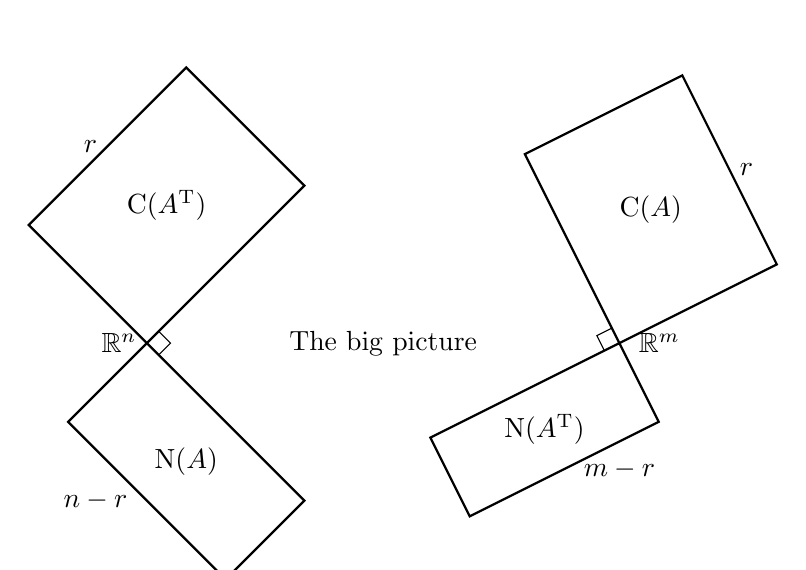
\begin{tikzpicture}
        \node at(3, 0){The big picture};
        \draw[thick](0, 0)node[left]{$\RR^n$}--(2, 2)--(.5, 3.5)--(-1.5, 1.5)node[midway, left]{$r$}--(2, -2)--(1, -3)--(-1, -1)node[midway, left]{$n-r~$}--cycle;
        \draw(.15, .15)--(.3, 0)--(.15, -.15);
        \node at(.25, 1.75){$\C(A\tp)$};
        \node at(.5, -1.5){$\N(A)$};
        \draw[thick](6, 0)node[right]{$~\RR^m$}--(8, 1)--(6.8, 3.4)node[midway, right]{$r$}--(4.8, 2.4)--(6.5, -1)--(4.1, -2.2)node[midway, right]{$~m-r$}--(3.6, -1.2)--cycle; % +6
        \draw(5.905, .19)--(5.715, .095)--(5.81, -.095); % .03√10
        \node at(6.4, 1.7){$\C(A)$};
        \node at(5.05, -1.1){$\N(A\tp)$};
    \end{tikzpicture}
    \tikzchap $A$的四个子空间
\end{center}
\paragraph{矩阵的秩的不等式}参考:\url{https://zhuanlan.zhihu.com/p/55206421}
\begin{theorem}{}{}
	
\end{theorem}
\clearpage
\section{正交性}
将列向量看做矩阵,则向量$v$和$w$的内积可以看做$v\cdot w = v\tp w.$
\begin{definition}{向量的正交}{vector orthogonal}
	若$v\tp w=0$,则称$v$和$w$正交(orthogonal)。
\end{definition}
依定义,0和所有向量正交。
\begin{theorem}{正交的模}{}
	若$v,w$正交,则
	\begin{align}
		\norm v^2+\norm w^2=\norm{v+w}^2.
	\end{align}
\end{theorem}
\subsection{正交性}
\begin{definition}{子空间的正交}{subspace orthogonal}
	定义线性空间$L$的两个子空间$V,W$正交,若$V$中的每一个向量均和$W$中每一个向量正交。
\end{definition}
显然,若$L$的子空间$V,W$正交,则
\begin{align}
	\dim(L)\geqslant\dim(V)+\dim(W).
\end{align}
\begin{definition}{正交补}{orthogonal complement}
	子空间$V$的正交补(orthogonal complement)~$V^\perp$由所有同$V$正交的向量组成。
\end{definition}
只有0同时属于$V$和$V^\perp$。
\begin{theorem}{线性代数基本定理·二}{fundamental theorems of linear algebra II}
	在$\RR^n$中,$\N(A)=\C(A\tp)^\perp.$

	在$\RR^m$中,$\N(A\tp)=\C(A)^\perp.$
\end{theorem}
\begin{theorem}{分解}{resolve}
$\forall x\in\RR^n$均可以分解成
\[
	x=x_r+x_n,
\]
其中$x_r\in\C(A\tp),\enspace x_n\in\N(A)$,且这种分解是唯一的。
\end{theorem}
\prf 由
\[
	Ax=A(x_r+x_n)=Ax_r\in\C(A\tp)
\]
知,只需证明:
$\forall b\in\C(A\tp)$,存在唯一的$x_r\in\C(A\tp)$使得$Ax_r=b.$

若存在$x_r,x_r'\in\C(A\tp)$满足$Ax_r=Ax_r'$,则$x_r-x_r'$同时在$\C(A\tp)$和$N(A)$中,故$x_r-x_r'=0.$\qed
\paragraph{矩阵的可逆部分}
对于矩阵$A$,把$N(A)$和$\N(A\tp)$对应的行和列去掉之后总是一个$r$阶可逆矩阵。
\begin{center}
    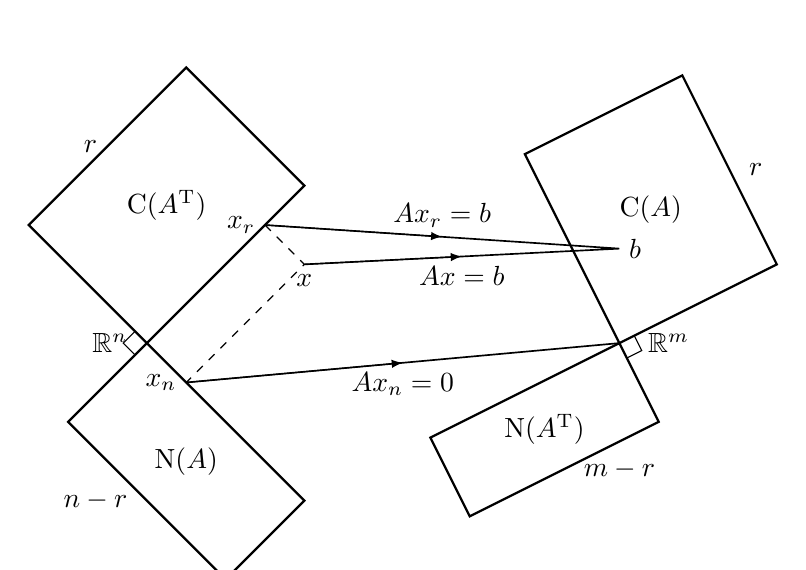
\begin{tikzpicture}
        \draw[thick](0, 0)node[left]{$\RR^n~$}--(2, 2)--(.5, 3.5)--(-1.5, 1.5)node[midway, left]{$r·$}--(2, -2)--(1, -3)--(-1, -1)node[midway, left]{$n-r~$}--cycle;
        \draw(-.15, .15)--(-.3, 0)--(-.15, -.15);
        \node at(.25, 1.75){$\C(A\tp)$};
        \node at(.5, -1.5){$\N(A)$};
        \draw[thick](6, 0)node[right]{$~~\RR^m$}--(8, 1)--(6.8, 3.4)node[midway, right]{$~r$}--(4.8, 2.4)--(6.5, -1)--(4.1, -2.2)node[midway, right]{$~m-r$}--(3.6, -1.2)--cycle; % +6
        \draw(6.19, .095)--(6.285, -.095)--(6.095, -.19); % .03√10
        \node at(6.4, 1.7){$\C(A)$};
        \node at(5.05, -1.1){$\N(A\tp)$};
        \coordinate[label=below:$x$](X)at(2, 1);
        \coordinate[label=left:$x_r$](R)at(1.5, 1.5);
        \coordinate[label=left:$x_n$](N)at(.5, -.5);
        \coordinate[label=right:$b$](B)at(6, 1.2);
        \draw[dashed](R)--(X)--(N);
        \draw[semithick](R)--(B)--(X);
        \draw[semithick](N)--(6, 0);
        \draw[-latex](R)--(3.75, 1.35)node[above]{$Ax_r=b$};
        \draw[-latex](X)--(4, 1.1)node[below]{$Ax=b$};
        \draw[-latex](N)--(3.25, -.25)node[below]{$Ax_n=0$};
    \end{tikzpicture}
    \tikzchap big picture升级版
\end{center}
\subsection{投影}
考虑向量$b$在向量$a$上的投影$p$
\[
	p=(\hat a\cdot b)\hat a=\frac{a\tp b}{a\tp a}a=\frac{aa\tp}{a\tp a}b.
\]
考虑$\RR^m$中线性无关的$n$个向量$(a_1,\ldots,a_n)=:A$张成的子空间,找到向量$p$在上面的投影
\[
	p=Ax=x_1a_1+\cdots+x_na_n\in\C(A).
\]
考虑投影的性质:$p$的终点在子空间中距离$b$的端点最近,则$(b-p)$同子空间垂直:
\[
	A\tp(b-Ax)=0
\]
相当于求解线性方程组
\[
	A\tp Ax=A\tp b.
\]
若$A\tp A$可逆,则$x=(A\tp A)\iv A\tp b$,由$p=Ax$可定义投影矩阵(project matrix)
\begin{align}
	P=A(A\tp A)\iv A\tp.
\end{align}
投影矩阵有性质:$P^2=P$,这也是符合投影性质的。
\begin{theorem}{$A\tp A$的可逆性}{ATA inverse}
	$A\tp A$可逆$\iff A$的列之间线性无关。
\end{theorem}
\prf 只需证明$\N(A\tp A)=\N(A)$即可。

$\forall x\in\N(A),\enspace Ax=0$,左乘$A\tp$得:$A\tp Ax=0,\enspace x\in\N(A\tp A)$;

$\forall x\in\N(A\tp A),\enspace A\tp Ax=0$,左乘$x\tp$得:$x\tp A\tp Ax=\norm{Ax}^2=0$,即$Ax=0,\enspace x\in\N(A)$。\qed

推论:
\[
	\rank(A)=\rank(A\tp)=\rank(A\tp A)=\rank(AA\tp).
\]
\subsection{最小二乘法}
考虑线性方程组$Ax=b$,$A$的行列$m>n$甚至$m\gg n$,一般来说无解。但仍可找到$x$使得$\norm{b-Ax}$最短。

由投影的性质,若$Ax$是$b$在$\C(A)$上的投影,则$\norm{b-Ax}$最短,此时
\[
	x=(A\tp A)\iv A\tp b.
\]
\begin{method}{直线拟合(最小二乘法)}{}
	$m$组数据$(x_i,y_i)$,确定线性关系$y=a+bx$中的系数$a,b$,即 
	\[
		\begin{bmatrix}
			1&x_1\\\vdots&\vdots\\1&x_m
		\end{bmatrix}
		\begin{bmatrix}
			a\\b
		\end{bmatrix}=
		\begin{bmatrix}
			y_1\\\vdots\\y_m
		\end{bmatrix},\quad\rightarrow\quad Ax=b.
	\]
	$\rank(A)=2$,故$A\tp A$可逆,
	\[
		A\tp A=
		\begin{bmatrix}
			n&(x_i)\\
			(x_i)&(x_i^2)
		\end{bmatrix},\quad
		(A\tp A)\iv=\frac1{m(x_i^2)-(x_i)^2}
		\begin{bmatrix}
			(x_i^2)&-(x_i)\\
			-(x_i)&m
		\end{bmatrix}.
	\]
	在此处$(x_i)$特指对$x_i$求和,得到 
	\[
		\begin{cases}
			a=\frac{(x_i^2)(y_i)-(x_i)(x_iy_i)}{m(x_i^2)-(x_i)^2}\\
			b=\frac{-(x_i)(y_i)-m(x_iy_i)}{m(x_i^2)-(x_i)^2}
		\end{cases}
	\]
	\iffalse
	\[
		A\tp A=
		\begin{bmatrix}
			n&\textstyle\sum_{i=1}^n x_i\\
			\textstyle\sum_{i=1}^n x_i&\textstyle\sum_{i=1}^n x_i^2
		\end{bmatrix}
	\]
	则
	\[
		(A\tp A)\iv=\frac1{\textstyle{n\sum_{i=1}^n x_i^2-\bigkh{\sum_{i=1}^n x_i}^2}}
		\begin{bmatrix}
			\textstyle\sum_{i=1}^n x_i^2&-\textstyle\sum_{i=1}^n x_i\\
			-\textstyle\sum_{i=1}^n x_i&n
		\end{bmatrix}
	\]
	得到 
	\[
		\begin{cases}
			a=\frac{\textstyle\sum_{i=1}^n x_i^2\sum_{i=1}^n y_i-\sum_{i=1}^n x_i\sum_{i=1}^n x_iy_i}{\textstyle{n\sum_{i=1}^n x_i^2-\bigkh{\sum_{i=1}^n x_i}^2}}\\[2ex]
			b=\frac{\textstyle-\sum_{i=1}^n x_i\sum_{i=1}^n y_i-n\sum_{i=1}^n x_iy_i}{\textstyle{n\sum_{i=1}^n x_i^2-\bigkh{\sum_{i=1}^n x_i}^2}}
		\end{cases}
	\]
	\fi
\end{method}
\begin{method}{多项式拟合}{}
	$m$组数据$(x_i,y_i)$,确定多项式关系
	\[
		y=a_0+a_1x+\cdots+a_nx^n
	\]
	中的系数$a_0,\ldots,a_n$,即 
	\[
		\begin{bmatrix}
			1&x_1&\cdots&x_1^n\\\vdots&\vdots&\ddots&\vdots\\1&x_m&\cdots&x_m^n
		\end{bmatrix}
		\begin{bmatrix}
			a_0\\\vdots\\a_n
		\end{bmatrix}=
		\begin{bmatrix}
			y_1\\\vdots\\y_m
		\end{bmatrix},\quad\rightarrow\quad Ax=b.
	\]
	从而$x=(A\tp A)\iv A\tp b.$
\end{method}
一般最小二乘拟合:……

两组数据相关不一定代表有因果。
\subsection{正交基、Gram-Schmidt法则、\textit{QR}分解}
基是一组线性无关的向量并且张成整个线性空间,我们对基之间的夹角和长度并没有要求。为了方便,我们可以要求基具备一些额外的性质。
\begin{definition}{正交归一基}{orthonomal basis}
	基$\{q_1,\ldots,q_n\}$是正交归一的(orthonomal)的,若 
	\[
		q_i\cdot q_j=\delta_{ij}
	\]
\end{definition}
将一组正交归一基$\{q_1,\ldots,q_n\}$按列排成矩阵$Q$,则$Q\tp Q=I$,称为正交矩阵(orthogonal matrix)。特别的,若$Q$是方阵,则
\[
	Q\tp=Q\iv,
\]
则$Q\tp Q=QQ\tp=I$,便得到正交归一基的完备性(complete)
\[
	\sum_{i=1}^nq_iq_i\tp=I.
\]
\begin{example}{Fourier级数}{Fourier series}
	定义函数$f,g$在$[-\pi,\pi]$上的内积
	\[
		\inp fg:=\int_{-\pi}^\pi f(x)g(x)\d x
	\]
	则三角函数系列
	\[
		\hkh{\frac1{\sqrt{2\pi}},\frac{\sin\theta}{\sqrt\pi},\frac{\cos\theta}{\sqrt\pi},\frac{\sin2\theta}{\sqrt\pi},\frac{\cos2\theta}{\sqrt\pi},\ldots}
	\]
	构成一组正交归一基,任意$[-\pi,\pi]$上平方可积的函数均可被展开为Fourier级数(Fourier series):
	\[
		f(x)=\frac{a_0}2+\sum_{n=1}^\infty(a_n\cos nx+b_n\sin nx).
	\]
	Fourier系数
	\[
		\begin{cases}
			a_n:=\frac1\pi\int_{-\pi}^\pi f(x)\cos nx\d x\\
			b_n:=\frac1\pi\int_{-\pi}^\pi f(x)\sin nx\d x
		\end{cases}
	\]
\end{example}
给定一组基$\{a_1,\ldots,a_n\}$,如何构造一组正交归一基$\{q_1,\ldots,q_n\}$?
\begin{method}{Gram-Schmidt法则}{Gram-Schmidt rule}
	\begin{compactenum}
		\item 选取$b_1:=a_1;$
		\item 从$a_2$减去沿着$b_1$方向的分量,作为$b_2$
		\[
			b_2:=a_2-\frac{b_1\tp a_2}{b_1\tp b_1}b_1;
		\]
		\item 从$a_i$减去沿着$b_1,\ldots,b_{i-1}$方向的分量,作为$b_i$
		\[
			b_i:=a_i-\sum_{j=1}^{i-1}\frac{b_j\tp a_i}{b_j\tp b_j}b_j.
		\]
	\end{compactenum}
	再归一化$\{b_1,\ldots,b_n\}$
	\[
		q_i:=\frac{b_i}{\norm{b_i}}.
	\]
\end{method}
若$m\times n$矩阵$A=(a_1,\ldots,a_n)$的列之间线性无关,可用Gram-Schmidt法则构造一组正交归一基$\{q_1,\ldots,q_n\}$,$q_i$同$a_1,\ldots,a_{i-1}$正交,定义
\[
	R:=Q\tp A=\begin{bmatrix}
		q_1\tp a_1&q_1\tp a_2&\cdots&q_1\tp a_n\\[1ex]
		0&q_2\tp a_2&\cdots&q_2\tp a_n\\
		0&0&\ddots&\vdots\\
		0&0&0&q_n\tp a_n
	\end{bmatrix}
\]
$R$是个上三角矩阵,故$A$可以写成正交矩阵和上三角矩阵的乘积:
\begin{equation}
	A=QR.
\end{equation}

在最小二乘法等应用中,$A\tp A=R\tp R$
\[
	x=(A\tp A)\iv A\tp b=R\iv Q\tp b.
\]
效率更高。
\clearpage
\section{行列式}
在例~\ref{exm:inverse of 2x2 matrix}~中,2阶方阵的逆为
\begin{align*}
	\begin{bmatrix}
		a&b\\c&d
	\end{bmatrix}\iv=\frac1{ad-bc}
	\begin{bmatrix}
		d&-b\\
		-c&a
	\end{bmatrix}.
\end{align*}
定义2阶方阵的行列式(determinant)
\begin{align}
	\det (A)\equiv\abs A\equiv\begin{vmatrix}
		a&b\\c&d
	\end{vmatrix}:=ad-bc.
\end{align}
特别的,给出3阶方阵的行列式
\begin{align}
	\begin{vmatrix}
		a_{11}&a_{12}&a_{13}\\
		a_{21}&a_{22}&a_{23}\\
		a_{31}&a_{32}&a_{33}
	\end{vmatrix}={}&a_{11}
	\begin{vmatrix}
		a_{22}&a_{23}\\
		a_{32}&a_{33}
	\end{vmatrix}-a_{12}
	\begin{vmatrix}
		a_{21}&a_{23}\\
		a_{31}&a_{33}
	\end{vmatrix}+a_{13}
	\begin{vmatrix}
		a_{21}&a_{22}\\
		a_{31}&a_{32}
	\end{vmatrix}\\\notag
	={}&a_{11}a_{22}a_{33}+a_{12}a_{23}a_{31}+a_{13}a_{21}a_{32}\\\notag
	&-(a_{13}a_{22}a_{31}+a_{11}a_{23}a_{32}+a_{12}a_{21}a_{33}).
\end{align}
\subsection{行列式}
下面我们用递归的方式给出行列式的定义。首先引入代数余子式。
\begin{definition}{代数余子式}{cofactor}
	对于$n$阶方阵$A$,记$A_{\neq ij}$为去掉第$i$行第$j$列得到的$(n-1)$阶方阵。则$A$的余子式(minor)定义为
	\begin{align}
		M_{ij}:=\det (A_{\neq ij});
	\end{align}
	代数余子式(cofactor)定义为
	\begin{align}
		C_{ij}:=(-)^{i+j}M_{ij}.
	\end{align}
\end{definition}
代数余子式前的正负号与矩阵中元素所在位置的关系:
\begin{align}
	\begin{bmatrix}
		+&-&+&\cdots\\
		-&+&-&\cdots\\
		+&-&+&\cdots\\
		\vdots&\vdots&\vdots&\ddots\\
	\end{bmatrix}
\end{align}
\begin{definition}{行列式}{determinant}
	
	$A$的行列式定义为:
	\begin{compactenum}
		\item $n=1$时,$\det (A)=a_{11};$
		\item $n>1$时,行展开或列展开(Laplace展开)
		\begin{align}
			\det (A) = \sum_{i=1}^na_{ij}C_{ij} = \sum_{\ell=1}^na_{k\ell}C_{k\ell}.
		\end{align}
	\end{compactenum}
\end{definition}
易得,单位矩阵行列式$\det I=1$,对角矩阵行列式
\begin{align}
	\det(\diag(a_1,\ldots,a_n))=a_1\cdots a_n.
\end{align}
\begin{theorem}{三角矩阵的行列式}{determinant of triangular matrix}
	三角矩阵的行列式等于对角元的乘积。
\end{theorem}
按行列式的定义进行计算即证。
\subsection{行列式的性质}
行列式可看做$n$个$n$维向量到数域$\FF$的映射:
\[
	\det (A)=T(a_1,\ldots,a_n),
\]
由定义,行列式是线性的:
\begin{compactenum}
	\item $T(a_1,\ldots,ka_i,\ldots,a_n)=kT(a_1,\ldots,a_i,\ldots,a_n);$
	\item $T(\ldots,a_i+b_i,\ldots)=T(\ldots,a_i,\ldots)+T(\ldots,b_i,\ldots).$
\end{compactenum}
除了线性,行列式还满足初等变换相关的性质:
\begin{compactenum}
	\item[3.] 交换$A$任意两行或两列得到$B$,则$\det(B)=-\det(A);$
	
	其推论是,若$A$中有任意两行或两列相同,则$\det(A)=0.$
	\item[4.] 将$A$的第$i$行乘一个常数加到第$j$行得到$B$,则$\det(A)=\det(B).$
	
	其推论是,若$A$的行/列之间线性相关,或者说秩小于阶,则$\det (A)=0.$
\end{compactenum}
因此$A$可逆$\enspace\Leftrightarrow\enspace\det(A)\neq 0.$
\begin{definition}{全反对称张量}{Levi-Civita symbol}
	定义全反对称张量(Levi-Civita symbol)~$\epsilon_{i_1\cdots i_n}$,其中$i_1,\ldots,i_n$取值范围$1,\ldots,n$,满足
	\begin{compactitem}
		\item $\epsilon_{1\cdots n}=1;$
		\item $\epsilon_{\cdots i_p\cdots i_q\cdots}=-\epsilon_{\cdots i_q\cdots i_p\cdots};$
		\item 任两个指标相同则$\epsilon_{\cdots i_p\cdots i_p\cdots}=0.$
	\end{compactitem}
	如果$i_1,\ldots,i_n$是$1,\ldots,n$的一个全排列,其从$1,\ldots,n$变换而来需要两两交换的次数为$p$,则 
	\[
		\epsilon_{i_1\cdots i_n}=(-1)^p.
	\]
\end{definition}
利用全反对称张量,行列式也可以定义为
\begin{align}
	\det(A)=\sum_{i_1,\ldots,i_n=1}^n\epsilon_{i_1\cdots i_n}a_{1i_i}\cdots a_{ni_n}.
\end{align}
或者进行一个抽象的定义:行列式$\det(A)=T(a_1,\ldots,a_n)$是$n$个$n$维向量到数域$\FF$的映射,且满足以下三个性质:
\begin{compactenum}
	\item $\det I=1;$
	\item 任意交换两列,行列式反号;
	\item 线性$\ldots$
\end{compactenum}
\subsection{行列式的运算}
\paragraph{行列式与矩阵运算}
行列式在矩阵转置下不变
\[
	\det(A\tp)=\det(A),
\]
\begin{theorem}{行列式与矩阵乘法}{determinant of multiplication}
	\begin{equation}
		\det(AB)=\det(A)\det(B).
	\end{equation}
\end{theorem}
\prf 若$A$不可逆,则$AB$不可逆,等式成立:
\[
	\det(AB)=\det(A)\det(B)=0.
\]
若$A$可逆,则可表示为一系列初等矩阵的乘积$A=E_k\cdots E_1$,从而
\begin{align*}
	&\det(AB)=\det(E_k\cdots E_1B)=\det(E_k)\det(E_{k-1}\cdots E_1B)\\
	&=\det(E_k)\cdots\det(E_1)\det(B)=\det(E_k\cdots E_1)\det(B)=\det(A)\det(B).\rqed
\end{align*}
其一个推论是
\begin{align}
	\det(A\iv)=\det(A)\iv.
\end{align}

但是行列式与矩阵加法之间并无必然联系:
\begin{align}
	\det(A+B)\neq\det(A)+\det(B).
\end{align}
但是当$A,B$满足特殊的条件时,$\det(A+B)$可以化简,见后文的定理~\ref{thm:matrix determinant lemma}。
\begin{theorem}{分块矩阵的行列式·一}{determinant of bolck matrix I}
	若$A$是$m$阶方阵,$D$是$n$阶方阵,$B$是$m\times n$矩阵,则
	\begin{align}
		\begin{vmatrix}
			A&B\\0&D
		\end{vmatrix}=\abs A\abs D.
	\end{align}
\end{theorem}
\prf 对$A,D$进行$LU$分解,$A=L_AU_A,D=L_DU_D$,则
\[
	\begin{bmatrix}
		A&B\\0&D
	\end{bmatrix}=
	\begin{bmatrix}
		L_A\\ &L_D
	\end{bmatrix}
	\begin{bmatrix}
		U_A&L_A\iv B\\ &U_D
	\end{bmatrix}
\]
前者为下三角矩阵,后者为上三角矩阵,故
\[
	\begin{vmatrix}
		A&B\\0&D
	\end{vmatrix}=\abs{L_A}\abs{L_D}\abs{U_A}\abs{U_D}=\abs A\abs D.\rqed
\]
\begin{theorem}{分块矩阵的行列式·二}{determinant of bolck matrix II}
	若$A$是$m$阶方阵,$D$是$n$阶方阵,且$A,D$至少一个可逆,$B$是$m\times n$矩阵,$C$是$n\times m$矩阵,则
	\begin{align}
		\begin{vmatrix}
			A&B\\C&D
		\end{vmatrix}=
		\abs A\abs{D-CA\iv B}=
		\abs D\abs{A-BD\iv C}
	\end{align}
\end{theorem}
\prf 注意到
\begin{align*}
	\begin{bmatrix}
		I&0\\-CA\iv&I
	\end{bmatrix}
	\begin{bmatrix}
		A&B\\C&D
	\end{bmatrix}&=
	\begin{bmatrix}
		A&B\\0&-CA\iv B+D
	\end{bmatrix};\\
	\begin{bmatrix}
		I&-BD\iv\\0&I
	\end{bmatrix}
	\begin{bmatrix}
		A&B\\C&D
	\end{bmatrix}&=
	\begin{bmatrix}
		A-BD\iv D&0\\C&D
	\end{bmatrix}.\rqed
\end{align*}
\begin{theorem}{\href{https://en.wikipedia.org/wiki/Matrix_determinant_lemma}{矩阵行列式引理}}{matrix determinant lemma}
	若$A$可逆且$u,v$均为$n$维列向量,则
	\begin{align}
		\det(A+uv\tp)=(1+v\tp A\iv u)\det(A).
	\end{align}
\end{theorem}
\prf 先证明命题对于$A=I$成立,事实上
\begin{align*}
	\begin{bmatrix}
		I\\v\tp&1
	\end{bmatrix}
	\begin{bmatrix}
		I+uv\tp&u\\ &1
	\end{bmatrix}
	\begin{bmatrix}
		I\\-v\tp&1
	\end{bmatrix}=
	\begin{bmatrix}
		I&u\\ &1+v\tp u
	\end{bmatrix}.
\end{align*}
故
\begin{align}
	\det(I+uv\tp)=1+v\tp u
\end{align}
进而 
\[
	\det(A+uv\tp)=\det(A)\det(I+A\iv uv\tp)=(1+v\tp A\iv u)\det(A).\rqed
\]
行列式的运算技巧不宜写得过多,因为这远非线性代数的精髓。
\subsection{Cramer法则、伴随矩阵}
\begin{theorem}{Cramer法则}{Cramer's rule}
	考虑线性方程组
	\[
		Ax=b,
	\]
	$Ae_i$是$A$的第$i$列,定义矩阵$B_i$为把$A$中第$i$列换为$b$的矩阵 
	\[
		B_i:=A[e_1,\ldots,e_{i-1},x,e_{i+1},\ldots,e_n],
	\]
	左右取行列式,则
	\begin{align}
		x_i=\frac{\det(B_i)}{\det(A)}.
	\end{align}
\end{theorem}
Cramer法则的应用之一是矩阵求逆,利用$AA\iv=I$,把$A\iv$的元素看做未知数,解线性方程组
\[
	(A\iv)_{ij}=\frac{C_{ji}}{\det(A)}.
\]
\begin{definition}{伴随矩阵}{adjoint matrix}
	$n$阶方阵$A$的伴随矩阵(adjoint matrix)~$\adj(A)$
	\begin{align}
		(\adj(A))_{ij}:=C_{ji}.
	\end{align}
\end{definition}
根据Cramer法则,
\begin{align}
	A\iv=\frac{\adj(A)}{\det(A)}.
\end{align}
特别注意,即使$A$不可逆,$\adj A$依然存在。
\begin{theorem}{伴随矩阵的性质}{characterist of adjoint}
	伴随矩阵与原矩阵可交换,其乘积为
	\begin{align}
		A\adj(A)=\adj(A)A=\det(A)I.
	\end{align}
\end{theorem}
\prf 根据Laplace展开
\begin{align*}
	\bigfkh{A\adj(A)}_{ij}&=\sum_{k}A_{ik}\bigfkh{\adj(A)}_{kj}=\sum_{k}(-)^{j+k}A_{ik}M_{jk}=\vd_{ij}\det(A);\\
	\bigfkh{\adj(A)A}_{ij}&=\sum_{k}\bigfkh{\adj(A)}_{ik}A_{kj}=\sum_{k}(-)^{i+k}M_{ki}A_{kj}=\vd_{ij}\det(A).%\rqed
\end{align*}
进而有
\[
	\det(A)\det\bigkh{\adj(A)}=\det\bigkh{\det(A)I}=\bigkh{\det(A)}^n.
\]
故伴随矩阵的行列式
\begin{align}
	\det\bigkh{\adj(A)}=\det(A)^{n-1}.
\end{align}
上面的性质并不要求$A$可逆。特别的,若$A$可逆,则伴随矩阵也可逆
\begin{align}
	\adj(A)\iv=\bigkh{\det(A)A\iv}\iv=\frac{A}{\det(A)},
\end{align}
伴随矩阵的伴随矩阵
\begin{align}
	\adj\bigkh{\adj(A)}=\bigkh{\adj(A)}\iv\det\bigkh{\adj(A)}=\bigkh{\det(A)}^{n-2}A.
\end{align}

最后评价一句Cramer法则:计算机运用Cramer法则解$n$元线性方程组的时间复杂度是$\bigo(n\cdot n!)$,且在数值上不稳定\footnote{Cramer, Gabriel (1750). "Introduction à l'Analyse des lignes Courbes algébriques" (in French). Geneva: Europeana. pp. 656-659. Retrieved 2012-05-18.},这是不可接受的。与其在计算方面的作用相比,其理论价值更为重大,即:研究了方程组的系数与方程组解的存在性与唯一性关系。
\clearpage
\section{特征值和特征向量}
\subsection{特征值和特征向量}
\begin{definition}{特征值和特征向量}{eigenvalue and eigenvector}
	方阵$A$的特征向量(eigenvector)~$x\neq 0$满足:
	\[
		Ax=\lambda x,\quad\lambda\in\FF.
	\]
	其中$\lambda$称为$A$的特征值(eigenvalue)。
\end{definition}
\begin{theorem}{特征值的性质}{}
	\begin{compactenum}
		\item $A$的特征向量$x$也是$A^n$的特征向量,特征值是$\lambda^n;$
		\item 若$A$可逆,则$x$也是$A\iv$的特征向量,特征值是$\lambda^{-1};$
		\item 三角矩阵的特征值就是对角元;
		\item $A$可逆$\enspace\Leftrightarrow\enspace A$所有特征值非0。
		
		只需注意到$A$可逆时$Ax=0$只有零解即可。
	\end{compactenum}
\end{theorem}
\begin{definition}{特征子空间}{eigen-subspace}
	$A$的所有特征值为$\lambda$的特征向量再加上0构成$\RR^n$的一个线性子空间,这个子空间就是$\N(A-\lambda I).$
\end{definition}
\begin{theorem}{特征值}{eigenvalue}
	假设$n$阶矩阵$A$有特征向量$x_1,\ldots,x_r$,对应特征值为$\lambda_1,\ldots,\lambda_r$,且这些特征值两两不等,则$x_1,\ldots,x_r$线性无关。
\end{theorem}
\prf 运用数学归纳法证明。$r=1$时,定理自动成立;

假设$r=m-1$定理成立,若定理在$r=m$时不成立,则
\begin{equation}
	\label{eqn:proof eigen 1}
	x_m=c_1x_1+\cdots+c_{m-1}x_{m-1},\tag{$\ast$}
\end{equation}
两边同时左乘$A$得
\begin{equation}
	\label{eqn:proof eigen 2}
	\lambda_mx_m=c_1\lambda_1x_1+\cdots+c_{m-1}\lambda_{m-1}x_{m-1},\tag{$\ast\ast$}
\end{equation}
$\lambda_m($\ref{eqn:proof eigen 1}$)-($\ref{eqn:proof eigen 2}$)$得,
\[
	0=c_1(\lambda_m-\lambda_1)x_1+\cdots+c_{m-1}(\lambda_m-\lambda_{m-1})x_{m-1},
\]
由$x_1,\ldots,x_{m-1}$线性无关可得所有的$c_i=0$,矛盾!\qed
\subsection{特征多项式}
求特征值$\lambda$需要解如下的特征方程(eigenfunction)
\[
	\det(\lambda I-A)=\lambda^n+a_1\lambda^{n-1}+\cdots+a_n=0,
\]
特别的,特征多项式(eigen-polynomial)的系数有如下性质:
\begin{align}
	a_1=-\tr(A),\quad a_n=(-)^n\det(A)
\end{align}
由Vieta定理,在考虑重根的情况下,
\begin{align}
	\tr(A)=\sum_{i=1}^n\lambda_i,\quad \det(A)=\prod_{i=1}^n\lambda_i.
\end{align}
更一般的,\href{https://en.wikipedia.org/wiki/Cayley%E2%80%93Hamilton_theorem}{Cayley-Hamilton定理}给出了其他项的系数表达式,比如
\[
	a_2=\frac12\bigkh{\tr^2(A)-\tr(A^2)}.
\]
\begin{theorem}{相似变换的特征多项式}{}
	$A$的相似变换$B\iv AB$和$A$有相同的特征多项式。
\end{theorem}
\prf 对下式两边取行列式即证
\[
	\lambda I-B\iv AB=B\iv(\lambda I-A)B.\rqed
\]
直接推论是:相似变换与原矩阵的迹相同
\begin{equation}
	\tr(B\iv AB)=\tr(A).
\end{equation}
\newpage
\subsection{矩阵对角化}
\begin{theorem}{可对角化判定}{}
	$n$阶矩阵$A$可对角化$\enspace\Leftrightarrow\enspace A$有$n$个线性无关的特征向量$x_1,\ldots,x_n$,此时$A=X\Lambda X\iv$,且 
	\begin{align}
		X=(x_1,\ldots,x_n),\quad\Lambda=\diag(\lambda_1,\ldots,\lambda_n).
	\end{align}
\end{theorem}
\prf 假设$A$有$n$个线性无关的特征向量$x_1,\ldots,x_n$,
\[
	AX=(Ax_1,\ldots,Ax_n)=(\lambda_1x_1,\ldots,\lambda_nx_n)=X\Lambda,
\]
故$A$可对角化;反过来说,若$A$可对角化为$X\Lambda X\iv$,则$AX=X\Lambda$,即
\[
	(Ax_1,\ldots,Ax_n)=(\lambda_1x_1,\ldots,\lambda_nx_n),
\]
故$x_1,\ldots,x_n$是$A$的特征向量,又$X$可逆,故$x_1,\ldots,x_n$线性无关。\qed

推论:有$n$个互不相同特征值的$n$阶矩阵$A$可对角化。当特征值重复时,引入两个概念
\begin{definition}{几何重数和代数重数}{}
	几何重数(geometric multiplicity, GM):特征值$\lambda$对应的最大线性无关的特征向量的个数,即$\dim\bigkh{\N(\lambda I-A)}$。

	代数重数(algebraic multiplicity, AM):特征值$\lambda$作为特征方程$\det(\lambda I-A)=0$的根的重复次数。
\end{definition}
特征方程可以写成
\[
	\prod_{i=1}^r(\lambda-\lambda_i)^{m_i}=0,
\]
其中$\lambda_i$是互不相同的根,$m_i$是$\lambda_i$的代数重数。
\begin{theorem}{}{GM <= AM}
	GM $\leqslant$ AM.
\end{theorem}
\prf 考虑$n$阶矩阵$A$,假设特征值$\lambda_1$的GM $=\dim(\lambda_1I-A)=m$,

取$\{x_1,\ldots,x_m\}$为$\C(\lambda_1I-A)$的一组正交归一基。

取$\{b_1,\ldots,b_{n-m}\}$为$\N(\lambda_1I-A)^\perp$的一组正交归一基。

设$n\times n$矩阵 
\[
	P=(x_1,\ldots,x_m,b_1,\ldots,b_{n-m})=(X,B),
\]
$P$是可逆的且$P\iv=P\tp$,且$X\tp B=0$,则 
\[
	P\iv AP=\begin{bmatrix}
		\lambda_1I_m&X\tp AB\\0&B\tp AB
	\end{bmatrix},
\]
分块三角矩阵
\[
	\det(\lambda I-P\iv AP)=(\lambda-\lambda_1)^m\det(\lambda I-B\tp AB),
\]
$A$和$P\iv AP$有相同的特征方程,故$\lambda_1$必然是$A$的特征方程的根,且其AM $\geqslant$ GM。\qed

推论:$n$阶矩阵$A$的全部特征值为$\{\lambda_1,\ldots,\lambda_r\}$,$A$可对角化当且仅当
\[
	\sum_{i=1}^r\dim(\lambda_iI-A)=n,
\]
即所有特征值的AM = GM。
\begin{theorem}{同时对角化}{}
	若$A,B$可对角化,则他们可以同时对角化当且仅当$AB=BA$。
\end{theorem}
\prf 若$A,B$可以同时对角化,故
\[
	A=X\Lambda_AX\iv,\quad B=X\Lambda_BX\iv,
\]
故
\[
	AB-BA=X(\Lambda_A\Lambda_B-\Lambda_B\Lambda_A)X\iv=0;
\]

若$AB=BA$,下证$A,B$可同时对角化。

设$A$的特征值为$\{\lambda_1,\ldots,\lambda_s\}$,$\lambda_i$对应特征子空间为$V_i$,几何重数$m_i=\dim(V_i)$,%为方便,
记$n_i:=m_1+\cdots+m_{i-1}$,
取$\{v_{n_i+1},\ldots,v_{n_i+m_i}\}$表示$V_i$的一组基,记$X=(v_1,\ldots,v_n)$,则$X$可对角化$A$
\[
	X\iv AX=\begin{bmatrix}
		\lambda_1I_{m_1}\\ &\ddots\\ &&\lambda_sI_{m_s}
	\end{bmatrix},
\]
$\forall x\in V_i$,
\[
	(AB-BA)x=(A-\lambda_iI)Bx=0,
\]
故$Bx\in V_i$,从而$X\iv BX$和$X\iv AX$一样是分块对角的:
\[
	X\iv BX=\begin{bmatrix}
		B_1\\ &\ddots\\ &&B_s
	\end{bmatrix},
\]
其中$B_i$是$m_i\times m_i$的。给定$B$的特征值$\xi_j$,其必是$B_1,\ldots,B_s$其中至少一个的特征值,不妨考虑$\xi_j$是$B_i$的特征值\footnote{无需考虑$\N(B_i)$},若$\xi_j$的AM $>B_i$的GM,则$\xi_j$的AM $>B$的GM,$B$便不能被对角化,与前提矛盾!故$B_i$均可被特定的$Y_i$对角化,即$Y_i\iv B_iY_i=\Lambda_i$,构造
\[
	Y=\begin{bmatrix}
		Y_1\\ &\ddots\\ &&Y_s
	\end{bmatrix}
\]
则$Y\iv X\iv BXY$是对角化的,同时$Y\iv X\iv AXY$也是对角化的,取$Z=XY$,便可同时对角化$A,B$。\qed
\subsectionstar{Jordan标准型}
不是所有方阵都可以对角化,如果$n$阶矩阵$A$有$r<n$个线性独立的特征向量,怎么把$A$变成最接近对角矩阵的形式?

\begin{theorem}{Jordan标准型}{Jordan normal form}
	$n$阶矩阵$A$有$r$个特征值,则存在$B$,使得
	\[
		B^{-1}AB=\begin{bmatrix}
			J_1             \\
			 & \ddots       \\
			 &        & J_r
		\end{bmatrix},\quad
		J_i=\begin{bmatrix}
			\lambda_i & 1                              \\
			          & \lambda_i & \ddots             \\
			          &           & \ddots & 1         \\
			          &           &        & \lambda_i
		\end{bmatrix}
	\]
	其中$J_i$称为Jordan块,$\lambda_i$是$A$的第$i$个特征值。
\end{theorem}
\prf 其证明是线性代数的核心。其中一些概念需要等到第 \ref{sec:linear mapping} 章线性映射才会提及。先给出几个概念证明引理。
\begin{definition}{广义特征向量}{general eigenvector}
	线性映射$T:V\to V$的广义特征向量(general eigenvector) $v\in V$且$v\neq 0$,使得$(T-\lambda I)^kv=0$对某个正整数$k$成立。这里$I:V\to V$是恒等映射。

	使得$(T-\lambda I)^dv=0$成立的最小正整数$d$称为$v$的幂指数(exponent)。
\end{definition}
\begin{theorem}{}{}
	给定正整数$k$,广义特征方程$(T-\lambda I)^kv=0$有解当且仅当$\lambda$是$T$的特征值。
\end{theorem}
\prf 若$\lambda$是$T$的特征值,则$(T-\lambda I)v=0$,左乘$(T-\lambda I)^{k-1}$即可。

若$(T-\lambda I)^kv=0$有解,则$w=(T-\lambda I)^{k-1}v$满足$(T-\lambda I)w=0$,$\lambda$是$T$的特征值。\qed
\begin{theorem}{}{}
	令$u_i:=(T-\lambda I)^iv$,则$B=\{u_0,\ldots,u_{d-1}\}$是一组线性无关的向量。
\end{theorem}
\prf 设
\[
	\sum_{i=0}^{d-1}a_iu_i=\sum_{i=0}^{d-1}a_i(T-\lambda I)^iv=0,
\]
左乘$(T-\lambda I)^{d-1}$,左边只剩$a_0(T-\lambda I)^{d-1}v$,故$a_0=0$;

递推地左乘$(T-\lambda I)^{d-2},(T-\lambda I)^{d-3},\ldots$可得到所有系数为0,从而$u_0,\ldots,u_{d-1}$线性无关。\qed
\begin{theorem}{}{}
	\[
		Tu_j=\begin{cases}
			\lambda u_j+u_{j+1},&1\leqslant j<d-1\\
			\lambda u_j,&j=d-1\\
			0,&j>d-1
		\end{cases}
	\]
\end{theorem}
\prf $1\leqslant j<d-1$时,$(T-\lambda I)u_j=u_{j+1}$,即$Tu_j=\lambda u_j+u_{j+1}$。

$j=d-1$时,$(T-\lambda I)u_j=0$,即$Tu_j=\lambda u_j$;

$j>d-1$时,$u_j=0$。\qed
\begin{theorem}{}{}
	$X=\spn(B)$是$T$的不变子空间,即$T(X)\subset X$
\end{theorem}
\prf 由上式,$\forall u=a_0u_0+\cdots+a_{d-1}u_{d-1}\in X$
\[
	Tu=\sum_{i=0}^{d-2}a_i(\lambda u_i+u_{i+1})+a_{d-1}\lambda u_{d-1}\in X.\rqed
\]
因为$X$是$T$的不变子空间,我们可以把$T$看成是$X\to X$的线性映射。
取$B$作为$X$的一组基,则$T$在$B$下的表示矩阵为
\[
	T=\begin{bmatrix}
		\lambda\\ 1&\lambda\\ &\ddots&\ddots\\ &&1&\lambda
	\end{bmatrix}
\]
这与Jordan块在定理 \ref{thm:Jordan normal form} 中的定义仅仅是转置的差别。

接下来我们将证明$V$中存在一组基,$T$在这组基上的表示矩阵是分块对角的,而且每一块都是Jordan块的形式。
\begin{theorem}{}{}
	若$v_1,\ldots,v_r$是$T$的广义特征向量,且相应的幂指数是$d_i$,设 
	\[
		u_{ij}:=(T-\lambda_iI)^jv_i,\quad V_i:=\spn(u_{i0},\ldots,u_{id-1}).
	\]
	之前证明了$V_i$是$T$的不变子空间,且$T$在$V_i$上的表示矩阵是Jordan块。故
	$T$在$V_1\oplus\cdots\oplus V_r$上的表示矩阵是分块对角的,且每一块都是Jordan块的形式。
\end{theorem}
%\prf 平凡的。\qed
所以我们只要证明存在这样一组广义特征向量$v_1,\ldots,v_r$使得$V=V_1\oplus\cdots\oplus V_r$就可以证明Jordan标准型的定理。

假设$\lambda$是$T$的某个特征值。如果$T-\lambda I$可以写成Jordan块的形式,则$T$也可以写成Jordan块的形式。所以以下我们用$T-\lambda I$代替$T$,或者说,考虑有一个特征值是0的线性映射$T$。
\begin{theorem}{}{}
	设$K_i=\ker(T^i),\,U_i=\Im(T^i)$,则
	\[
		K_1\subset K_2\subset\cdots,\quad U_1\supset U_2\supset\cdots
	\]
\end{theorem}
\prf 
\clearpage
\subsection{对称矩阵}
\begin{theorem}{对称矩阵的性质·一}{characterist of sysmmetric matrix I}
	若$S$是一个$n$阶实对称矩阵,则$S$至少有一个实特征值$\lambda$
\end{theorem}
\prf 由代数基本定理,对任何矩阵,$S$的特征方程至少会得到一个复特征值$\lambda$,其对应的特征向量为$z$ (一般也是复的),则$\bar z\tp z>0$。
\[
	Sz=\lambda z,\quad S\bar z=\bar S\bar z=\overline{Sz}=\bar\lambda\bar z,
\]
由$S$的对称的性质,注意到
\[
	\bar z\tp Sz=\lambda\bar z\tp z=\lambda(\bar z\tp z)\tp=\lambda z\tp\bar z=(Sz)\tp\bar z=z\tp S\bar z=\bar\lambda z\tp\bar z.
\]
故$\lambda=\bar\lambda$.\qed

由代数基本定理的递归性,可推知$S$的所有特征值都是实数。
\begin{theorem}{对称矩阵的性质·二}{characterist of sysmmetric matrix II}
	$v$是$S$的特征向量,若$w\perp v$,则$Sw\perp v$。
\end{theorem}
\prf 
\[
	(Sw)\tp v=w\tp S\tp v=w\tp Sv=\lambda w\tp v=0,\rqed
\]
\begin{theorem}{对称矩阵的性质·三}{characterist of sysmmetric matrix III}
	若$W$是$\RR^n$的一个线性子空间且在$S$的作用下稳定:
	\[
		\forall w\in W,\enspace Sw\in W,
	\]
	则$W^\perp$在$S$的作用下稳定:
	\[
		\forall u\in W^\perp,\enspace Su\in W^\perp.
	\]
\end{theorem}
\prf $\forall w\in W,u\in W^\perp$
\[
	(Su)\tp w=u\tp S\tp w=u\tp(Sw)=0.\rqed
\]
\begin{theorem}{谱定理}{spectral theorem}
	对称矩阵$S$总可以被一个正交矩阵$Q$对角化。
\end{theorem}
\prf 由定理 \ref{thm:characterist of sysmmetric matrix I} 和推论可知$S$至少有一个实特征值$\lambda_1$和实特征向量$q_1$且$q_1\tp q_1=1$,$S$在$q_1$张成的一维线性空间上是稳定的。

由定理 \ref{thm:characterist of sysmmetric matrix III} 可知$S$作用在$\C(q_1)^\perp$上也是稳定的,假设$\C(q_1)^\perp$上有一组正交归一基为$\{a_1,\ldots,a_{n-1}\}$,构造矩阵$X_1=[q_1,a_1,\ldots,a_{n-1}]$,且$X$是正交的$X_1\tp X_1=I$,
\[
	X_1\tp SX_1=X_1\tp[\lambda q_1,Sa_1,\ldots,Sa_{n-1}]=\begin{bmatrix}
		\lambda_1\\ &S_1
	\end{bmatrix}.
\]
$S_1$是一个$(n-1)$阶方阵,且$(S_1)_{ij}=a_i\tp Sa_j$的,显然它也是对称的。

重复上述步骤,直到用$S$的特征向量构造出$\RR^n$的一组正交归一基:

对$S_1$可构造$(n-1)$阶的正交矩阵$X_2$,使得
\[
	X_2\tp S_1X_2=\begin{bmatrix}
		\lambda_2\\ &S_2
	\end{bmatrix},
\]
其中$S_2$是一个$(n-2)$阶对称方阵。从而
\[
	\begin{bmatrix}
		1\\ &X_2\tp
	\end{bmatrix}X_1\tp SX_1\begin{bmatrix}
		1\\ &X_2
	\end{bmatrix}=\begin{bmatrix}
		\lambda_1\\ &\lambda_2\\ &&S_2
	\end{bmatrix}.
\]
$Q_2:=X_1\diag(1, X_2)$也是正交的……最终有
\[
	Q_n\tp SQ_n=\begin{bmatrix}
		\lambda_1\\ &\ddots\\ &&\lambda_n
	\end{bmatrix}.
\]
$Q_n$也是正交的。\qed

对角化对称矩阵$S$的正交矩阵$Q$可被构造:
\begin{compactitem}
	\item 若$S$的特征值互不相同,对应的归一特征向量$q_i$两两正交,可选$Q=[q_1,\ldots,q_n]$;
	\item 若$S$的特征值有重复,取$\{q_i\}$为相应特征子空间的正交基。
\end{compactitem}
\subsection{正定矩阵}
\begin{definition}{二次型}{quadratic form}
	二次型(quadratic form)是形如$x\tp Sx$的二次多项式,其中$S$是实对称矩阵。
\end{definition}
\begin{definition}{正定矩阵}{positive definite matrix}
	给定对称矩阵$S$,如果$\forall x\neq 0$,二次型$x\tp Sx>0$,则称$S$是正定的(positive definite)。
\end{definition}
\begin{theorem}{正定矩阵的判定}{determination of positive definite matrix}
	对于对称矩阵$S$,下述命题是等价的:
	\begin{compactenum}
		\item $\forall x\neq 0$,二次型$x\tp Sx>0$;
		\item $S$的所有$n$个特征值都是正的;
		\item $S$可以只通过换行和倍加后得到$n$个正的主元;
		\item $S$的所有左上行列式(前$i$行$i$列子矩阵的行列式)均$>0$;
		\item 存在$A$列之间线性无关,使得$S=A\tp A$。
	\end{compactenum}
\end{theorem}
\prf $1\Rightarrow 2$:$S$对称,则$\Lambda=Q\tp SQ$
\[
	\lambda_i=e_i\tp \Lambda e_i=e_i\tp Q\tp SQe_i=(Qe_i)\tp S(Qe_i)>0.
\]
$2\Rightarrow 1$:$S$的所有$n$个特征值都是正的,故
\[
	x\tp Sx=x\tp Q\Lambda Q\tp x=\sum_{i=1}^n\lambda_i(Q\tp x)^2_i>0.
\]
$5\Rightarrow 1$:$A$列之间线性无关,故$\forall x\neq 0,\enspace Ax\neq 0$
\[
	x\tp Sx=x\tp A\tp Ax=(Ax)\tp(Ax)>0.
\]
$1\Rightarrow 5$:$S$正定,故
\[
	S=Q\Lambda Q\tp=Q\begin{bmatrix}
		\sqrt{\lambda_1}\\ &\ddots\\ &&\sqrt{\lambda_n}
	\end{bmatrix}\begin{bmatrix}
		\sqrt{\lambda_1}\\ &\ddots\\ &&\sqrt{\lambda_n}
	\end{bmatrix}Q\tp=:A\tp A.
\]
$3\Rightarrow 4$:行倍加不改变所有左上行列式,$S$做行倍加得到上三角矩阵$U$,其$i\times i$的左上行列式就是前$i$个主元的乘积,所以$>0$。\\
$4\Rightarrow 3$:$U$的左上行列式都$>0$,所以前$i$个主元乘积都$>0$,所以主元全正。\\
$3\Rightarrow 5$:$S=LDU$,由$S$对称且$LDU$分解唯一可知$L=U\tp$,又主元全正,故
\[
	S=U\tp DU=U\tp\begin{bmatrix}
		\sqrt{a_1}\\ &\ddots\\ &&\sqrt{a_n}
	\end{bmatrix}\begin{bmatrix}
		\sqrt{a_1}\\ &\ddots\\ &&\sqrt{a_n}
	\end{bmatrix}U=:A\tp A.
\]
$5\Rightarrow 3$:$A$列之间线性无关,故$A=QR$
\[
	A\tp A=R\tp Q\tp QR=R\tp R=LDU.\rqed
\]
\begin{definition}{半正定矩阵}{positive semidefinite matrix}
	如果$\forall x\neq 0$,二次型$x\tp Sx\geqslant 0$,则称$S$是半正定的(positive semidefinite)。
\end{definition}
\begin{theorem}{半正定但非正定矩阵的判定}{determination of positive semi-but-not definite matrix}
	\begin{compactenum}
		\item $S$的最小特征值是0;
		\item 存在$A$列之间线性相关,使得$S=A\tp A$。
	\end{compactenum}
\end{theorem}
半正定但非正定矩阵的行列式为0.

\clearpage
\section{奇异值分解}
特征值和特征向量只适用于方阵,对于一般的$m\times n$矩阵$A$,有没有类似的操作?

考虑$A\tp A$和$AA\tp$,他们都是半正定的,因为$\forall x$
\[
	x\tp A\tp Ax=\norm{Ax}^2\geqslant 0,
\]
$AA\tp$同理,因此$A\tp A$和$AA\tp$都可以对角化。
\begin{definition}{奇异值}{singular value}
	$A\tp A$是半正定的,因此所有特征值$\lambda_i\geqslant 0$,矩阵$A$的奇异值(singular value)便定义为$A\tp A$特征值的平方根:$\sigma_i:=\sqrt{\lambda_i}$。

	为了后续方便,我们将所有奇异值从大到小排列:
	\[
		\sigma_1\geqslant\sigma_2\geqslant\cdots\geqslant\sigma_n\geqslant 0.
	\]
\end{definition}
由定理 \ref{thm:ATA inverse},$\rank(A\tp A)=\rank(A)$
\begin{theorem}{非零奇异值的数量}{number of non-zero singular value}
	$A$的非零奇异值的数量$r=\rank(A)$。
\end{theorem}
\prf 设$\{v_1,\ldots,v_n\}$为$\RR^n$中可以把$A\tp A$对角化的一组正交归一基,$\{\lambda_1,\ldots,\lambda_n\}$为对应的特征值,则$\{Av_1,\ldots,Av_n\}$是一个正交向量集合,即$\forall i\neq j$,
\[
	(Av_i)\tp Av_j=v_i\tp A\tp Av_j=v_i\tp(\lambda_jv_j)=0.
\]
假设$\lambda_1\geqslant\cdots\geqslant\lambda_r>0$是所有的正特征值,则$Av_{r+1},\ldots,Av_n=0$.

%因为$\{v_1,\ldots,v_n\}$为$\RR^n$中可以把$A\tp A$对角化的正交归一基,所以
$\forall x\in\RR^n$,$x$可以写成$x=c_1v_1+\cdots+c_nv_n$,
%因为$\C(A)$是由$A$所有列的线性组合得到的,所以
从而$\forall y\in\C(A)$,$y$可以被写为$\{Av_1,\ldots,Av_r\}$的线性组合:
\[
	y=Ax=c_1Av_1+\cdots+c_rAv_r+0+\cdots+0,
\]
故$\{Av_1,\ldots,Av_r\}$是$\C(A)$的一组正交基,$r=\rank(A)$。\qed
\subsection{奇异值分解}
\begin{theorem}{奇异值分解}{singular value resolve}
	$m\times n$矩阵$A$秩为$r$,则存在一个$m\times n$的矩阵$\Sigma$ 
	\[
		\Sigma=\begin{bmatrix}
			D&0\\0&0
		\end{bmatrix},\quad D=\diag(\sigma_1,\ldots,\sigma_r).
	\]
	$m\times m$的正交矩阵$U$和$n\times n$的正交矩阵$V$,且 
	\[
		A=U\Sigma V\tp.
	\]
\end{theorem}
\prf 直接构造出$U,\Sigma,V$。

$A\tp A$是对称矩阵,存在一组$\RR^n$中的正交归一基$\{v_1,\ldots,v_n\}$可将$A\tp A$对角化,$\{\lambda_1,\ldots,\lambda_n\}$为对应的特征值,且$\lambda_1,\ldots,\lambda_r>0,\enspace\lambda_{r+1},\ldots,\lambda_n=0.$

因为$\{v_1,\ldots,v_n\}$之间是正交的,则$\forall i\neq j$,
\[
	(Av_i)\tp(Av_j)=v_i\tp A\tp Av_j=\lambda_jv_i\tp v_j=0.
\]
所以$\{Av_1,\ldots,Av_r\}$之间也是正交的,$Av_{r+1},\ldots,Av_n=0$。令
\[
	u_i=\frac{Av_i}{\norm{Av_i}}=\frac{Av_i}{\sqrt{\lambda_i}}=\frac{Av_i}{\sigma_i},\quad i=1,\ldots,r.
\]
则$\{u_1,\ldots,u_r\}$是$\C(A)$的一组正交归一基。

再设$\{u_{r+1},\ldots,u_m\}$是$\N(A\tp)$中的一组正交归一基,因为$\N(A\tp)=\C(A)^\perp$,则$\{u_1,\ldots,u_m\}$是$\RR^m$的一组正交归一基。

设矩阵$U=(u_1,\ldots,u_m),\enspace V=(v_1,\ldots,v_n)$,$U$和$V$都是正交矩阵,且
\[
	AV=(Av_1,\ldots,Av_n)=(\sigma_1u_1,\cdots,\sigma_ru_r,0,\ldots,0)=U\Sigma.\rqed
\]
\begin{theorem}{}{ATA, AAT's singular value are same}
	$A\tp A$和$AA\tp$的非零特征值相同。
\end{theorem}
\prf 假设$x_i$是$A\tp A$的特征值为$\lambda_i\neq 0$的特征向量,
\[
	(\lambda_iI-A\tp A)x_i=0,
\]
左乘$A$,
\[
	A(\lambda_iI-A\tp A)x_i=(\lambda_iI-AA\tp)(Ax_i)=0,
\]
又$x_i\tp A\tp Ax_i=\lambda_i x_i\tp x_i>0$,所以$Ax_i\neq 0$,所以$Ax_i$是$AA\tp$的特征值为$\lambda_i$的特征向量。

同理,如果$x_i$是$AA\tp$的特征值为$\lambda_i\neq 0$的特征向量,$A\tp x_i$是$A\tp A$的特征值为$\lambda_i$的特征向量。

从而$A\tp A$和$AA\tp$非零特征值对应的特征向量一一对应。
\begin{example}{四个子空间的正交归一基}{}
	$\{v_1,\ldots,v_r\}$是$\C(A\tp)$的正交归一基,$V_r=(v_1,\ldots,v_r)$

	$\{v_{r+1},\ldots,v_n\}$是$\N(A)$的正交归一基,$V_{n-r}=(v_{r+1},\ldots,v_n)$

	$\{u_1,\ldots,u_r\}$是$\C(A)$的正交归一基,$U_r=(u_1,\ldots,u_r)$

	$\{v_{r+1},\ldots,v_n\}$是$\N(A\tp)$的正交归一基,$U_{n-r}=(u_{r+1},\ldots,v_m)$
\end{example}
\begin{example}{数据压缩}{}
	假设$\rank(A)<\min(m,n)$,则 
	\[
		A=[U_r,U_{m-r}]\begin{bmatrix}
			D&0\\0&0
		\end{bmatrix}\begin{bmatrix}
			V_r\tp\\V_{n-r}\tp
		\end{bmatrix}=U_rDV_r\tp=\sum_{i=1}^r\sigma_iu_iv_i\tp.
	\]
	可以用$U_r,D,V_r$这三个矩阵的$r(m+1+n)$个分量完全决定$A$原来的$mn$个分量。(无损)
	\tcblower
	甚至可以把很小的奇异值当成0,进一步压缩图片。(有损)由此带来的误差
	\[
		\vd A=\sum_{\ell=k+1}^r\sigma_\ell u_\ell v_\ell\tp.
	\]
	分量误差的绝对值
	\[
		|\vd A_{ij}|=\abs{\sum_{\ell=k+1}^r\sigma_\ell (u_\ell)_i (v_\ell)_j}\leqslant\sum_{\ell=k+1}^r\sigma_\ell.
	\]
	因此误差由忽略的奇异值控制,忽略的越少误差越小
\end{example}
\subsection{矩阵的模}
我们用内积定义了向量的模(即长度)
\[
	\norm x:=\sqrt{x\tp x}.
\]
\begin{theorem}{}{max Ax/x}
	\begin{equation}
		\norm{Ax}\leqslant\sigma_1\norm x.
	\end{equation}
\end{theorem}
\prf 
\begin{align*}
	\norm{Ax}^2&=x\tp A\tp Ax=x\tp V\Sigma\tp\Sigma V\tp x\\
	&=\sum_{k=1}^rx\tp v_k\sigma_k^2v_k\tp x\leqslant\sigma_1^2\sum_{k=1}^nx\tp v_kv_k\tp x\\
	&=\sigma_1^2x\tp VV\tp x=\sigma_1^2x\tp x,
\end{align*}
等号可在$x=cv_1$时成立。\qed
\begin{definition}{矩阵的模}{norm of matrix}
	矩阵的模(norm)定义为 
	\begin{equation}
		\norm A:=\max_{x\neq 0}\frac{\norm{Ax}}{\norm x}=\sigma_1.
	\end{equation}
\end{definition}
由矩阵模的定义可直接导出$\forall x\neq 0$,
\[
	\norm{Ax}\leqslant\norm A\norm x.
\]
\begin{theorem}{三角不等式}{triangle inequality}
	\begin{equation}
		\norm{A+B}\leqslant\norm A+\norm B.
	\end{equation}
\end{theorem}
\prf 
\[
	\norm{(A+B)x}=\norm{Ax+Bx}\leqslant\norm{Ax}+\norm{Bx}\leqslant\norm A\norm x+\norm B\norm x.
\]
故
\[
	\norm{A+B}=\max_{x\neq 0}\frac{\norm{(A+B)x}}{\norm x}\leqslant\norm A+\norm B.\rqed
\]
\begin{theorem}{Eckart-Young-Mirsky定理}{Eckart-Young-Mirsky theorem}
	同矩阵$A$最接近的秩为$k$的矩阵为
	\begin{equation}
		A_k=\sum_{i=1}^k\sigma_iu_iv_i\tp.
	\end{equation}
\end{theorem}
\prf 只需证$\forall B$秩为$k$,都有
\[
	\norm{A-B}\geqslant\norm{A-A_k}=\sigma_{k+1}.
\]
设$w=c_1v_1+\cdots+c_{k+1}v_{k+1}$,因为$\rank(B)=k$,故$Bv_1,\ldots,Bv_{k+1}$必然线性相关,继而存在非零的$c_1,\ldots,c_{k+1}$使得$Bw=0$,在此基础上再归一化$w$,从而
\begin{align*}
	\norm{A-B}^2&\geqslant\norm{(A-B)w}^2=\norm{Aw}^2\\
	&=\sigma_1^2c_1^2+\cdots+\sigma_{k+1}^2c_{k+1}^2\geqslant\sigma_{k+1}^2(c_1^2+\cdots+c_{k+1}^2)=\sigma_{k+1}^2.\rqed
\end{align*}
\subsection{伪逆}
\begin{definition}{伪逆}{pseudoinverse}
	$m\times n$矩阵$A=U\Sigma V\tp$,定义伪逆(pseudoinverse)是一个$n\times m$的矩阵
	\begin{equation}
		A^+:=V\Sigma^+U\tp.
	\end{equation}
	其中$\Sigma^+$是一个$n\times m$的矩阵
	\[
		\Sigma^+:=\begin{bmatrix}
			D\iv&0\\0&0
		\end{bmatrix},\quad D\iv=\diag(\sigma_1\iv,\ldots,\sigma_r\iv).
	\]
\end{definition}
伪逆与原矩阵的乘积并不是单位矩阵:
\[
	A^+A=V\begin{bmatrix}
		I_r&0\\0&0
	\end{bmatrix}V\tp,
\]
是投影到$\C(A\tp)$的矩阵;
\[
	AA^+=U\begin{bmatrix}
		I_r&0\\0&0
	\end{bmatrix}U\tp,
\]
是投影到$\C(A)$的矩阵。

但额外的满足:
\[
	AA^+A=A,\quad A^+AA^+=A^+.
\]
\begin{theorem}{伪逆与最小二乘法}{}
	最小二乘法
	\[
		A\tp Ax=A\tp b,
	\]
	的解为$x^+=A^+b$。
\end{theorem}
\prf 
\[
	A\tp Ax^+=V\Sigma\tp U\tp U\Sigma V\tp V\Sigma^+U\tp b=V\Sigma\tp U\tp b=A\tp b.\rqed
\]
\subsection{主成分分析}
一组数据$\mu=(\mu_1,\ldots,\mu_n)$来源于$n$个样本,其平均值(mean)和方差(variance)分别为
\[
	\bar\mu=\frac1n\sum_{i=1}^n\mu_i,\quad\sigma^2=\frac1{n-1}\sum_{i=1}^n(\mu_i-\bar\mu)^2.
\]
将数据存在一个$m\times n$的矩阵$A$中,每一行对应一种数据,每一列代表一个样本。将每个元素减去其所在行的平均值
\[
	A_{ij}:=(A_0)_{ij}-\frac1n\sum_{k=1}^n(A_0)_{ik}.
\]
由此得到矩阵$A$,每一行都是以0为中心的分布。
\begin{definition}{协方差矩阵}{covariance matrix}
	定义协方差矩阵(covariance matrix)
	\begin{equation}
		S:=\frac{AA\tp}{n-1}.
	\end{equation}
	对角线上$S_{ii}$是样本方差;$S_{ij}$是样本协方差。
\end{definition}
\begin{method}{主成分分析}{principal component analysis}
	主成分分析(principal component analysis, PCA):找到原有数据的一系列线性组合作为新的数据,新数据之间的协方差为0.
\end{method}
利用$A=U\Sigma V\tp$,定义新的数据矩阵$B:=U\tp A=\Sigma V$,$B$的协方差矩阵
\[
	\frac{BB\tp}{n-1}=\frac{\Sigma\Sigma\tp}{n-1}
\]
是对角的,故$B$之间协方差为0。

这种变换总方差是不变的:
\[
	\tr\biggkh{\frac{BB\tp}{n-1}}=\frac{\tr(U\tp AA\tp U)}{n-1}=\frac{\tr(UU\tp AA\tp)}{n-1}=\tr\biggkh{\frac{AA\tp}{n-1}}.
\]
所有数据点分布在$\{u_1,\ldots,u_r\}$张成的$\C(A)$上,$u_1$是所有数据变化最大的方向(方差最大)、$u_2$次之……$\{u_1,\ldots,u_r\}$称作主成分(principal component)。
\clearpage
\section{线性映射}
\label{sec:linear mapping}
\begin{definition}{映射}{mapping}
	$S,S'$是两个集合,如果$\forall x\in S$,均有一个$f(x)=x'\in S'$与之对应,这种对应关系$f:S\to S'$便叫映射(mapping)。

	$S$为定义域(domain of definition),$S'$为陪域(codomain)。$f(x)$叫做$x$在映射$f$下的像(image),$f(S)$为值域(domain of function)。
\end{definition}
\begin{definition}{映射的复合}{mapping composition}
	$f:U\to V,\enspace g:V\to W$,则$f,g$的复合(composition)构成一个新的映射$g\circ f:U\to W$,
	\[
		g\circ f(x)=g\bigkh{f(x)}.
	\]
\end{definition}
映射的复合满足结合律
\[
	(h\circ g)\circ f=h\circ (g\circ f)\equiv h\circ g\circ f.
\]
\begin{definition}{映射有关的概念}{mapping related concepts}
	映射$f:S\to S'$,$y$的原像(preimage)
	\[
		f\iv(y)=\set{x\in S}{f(x)=y}.
	\]
	单射(injection):$\forall x,y\in S$,$x\neq y$均有$f(x)\neq f(y)$。

	满射(surjection):$f(S)=S'$。

	双射(bijection):既是单射又是满射

	恒等映射(identity map):$\id:S\to S$,$\forall x\in S,\enspace\id(x)=x.$

	逆映射(inverse map):若存在$g:S'\to S$使得
	\[
		g\circ f=\id_S,\quad f\circ g=\id_{S'},
	\]
	则称映射$f:S\to S'$可逆,$g=f\iv$为$f$的逆。
\end{definition}
\begin{theorem}{可逆映射}{inverse}
	\begin{center}
		映射$f:S\to S'$可逆$\enspace\Leftrightarrow\enspace f$是双射。
	\end{center}
\end{theorem}
\prf 若$f$可逆,$g:S'\to S$为$f$的逆。若$x,y\in S$,满足$f(x)=f(y)$,则 
\[
	x=g\bigkh{f(x)}=g\bigkh{f(y)}=y.
\]
故$f$为单射;又$\forall z\in S'$,取$x=g(z)\in S$,可得$f(x)=f\bigkh{g(z)}=z$,故$f$为满射。

若$f$为双射,因为$f$为满射,$\forall z\in S'$,有$x\in S$使得$f(x)=z$,又因$f$为单射,因此$x$是唯一的,我们可以定义$g(z)=x$,故$g$是$f$的逆映射。\qed
\subsection{线性映射和矩阵}
\begin{definition}{线性映射}{linear mapping}
	$V,W$是两个线性空间,映射$T:V\to W$是线性映射(linear mapping)若$T$满足:
	\begin{compactenum}
		\item $\forall u,v\in V,\enspace T(u+v)=T(u)+T(v);$
		\item $\forall c\in\FF,\enspace T(cu)=cT(u).$
	\end{compactenum}
	线性映射也被称为线性变换;特别的,$V\to\RR$的称为线性函数。
\end{definition}
推论:$T(0)=0.$
\begin{theorem}{线性映射与基}{linear mapping and base}
	$V,W$是线性空间,$\{v_1,\ldots,v_n\}$是$V$中的一组基,$\{w_1,\ldots,w_n\}$是$W$中任意$n$个元素,则存在唯一的线性映射$T:V\to W$使得
	\[
		T(v_1)=w_1,\enspace\ldots,\enspace T(v_n)=w_n.
	\]
\end{theorem}
\prf (存在性) $\forall v\in V$均可唯一写成基的线性组合$v=c_1v_1+\cdots+c_nv_n$,定义映射$T:V\to W$
\[
	T(v)=c_1w_1+\cdots+c_nw_n,
\]
下面证明$T$是线性映射,再任取$u=d_1v_1+\cdots+d_nv_n\in V$
\begin{align*}
	T(v+u)&=T\bigkh{(c_1+d_1)v_1+\cdots+(c_n+d_n)v_n}\\
	&=(c_1+d_1)w_1+\cdots+(c_n+d_n)w_n=T(v)+T(u);\\
	T(cv)&=T(cc_1v_1+\cdots+cc_nv_n)=cc_1w_1+\cdots+cc_nw_n=cT(v).
\end{align*}
(唯一性) 假设存在另一个线性映射$F:V\to W$满足
\[
	F(v_1)=w_1,\enspace\ldots,\enspace F(v_n)=w_n,
\]
则 
\[
	F(v)=c_1F(v_1)+\cdots+c_nF(v_n)=c_1w_1+\cdots+c_nw_n=T(v).\rqed
\]
因此只要知道一个线性映射在基上的值,就唯一决定了整个线性映射。
\begin{example}{矩阵定义线性映射}{linear mapping defined by matrix}
	$m\times n$的矩阵$A$可定义一个线性映射$L_A:\RR^n\to\RR^m$,
	\[
		\forall x\in\RR^n,\enspace L_A(x)=Ax.
	\]
\end{example}
\begin{theorem}{线性映射和矩阵}{linear mapping and matrix}
	设$L:\RR^n\to\RR^m$是线性映射,则存在唯一的矩阵$A$使得$L=L_A$。
\end{theorem}
\prf 设$\{e_1,\ldots,e_n\}$是$\RR^n$的标准基,$\{f_1,\ldots,f_m\}$是$\RR^m$的标准基,$\forall x\in\RR^n$,有$x=x_1e_1+\cdots+x_ne_n$,则
\[
	L(x)=x_1L(e_1)+\cdots+x_nL(e_n).
\]
$L(e_i)\in\RR^m$,故可写成基的线性组合
\[
	L(e_i)=a_{1i}f_1+\cdots+a_{mi}f_m.
\]
故
\begin{align*}
	L(x)&=x_1(a_{11}f_1+\cdots+a_{m1}f_m)+\cdots+x_n(a_{n1}f_1+\cdots+a_{nm}f_m)\\
	&=(a_{11}x_1+\cdots+a_{1n}x_n)f_1+\cdots+(a_{m1}x_1+\cdots+a_{mn}x_n)f_m\\
	&=\begin{bmatrix}
		a_{11}x_1+\cdots+a_{1n}x_n\\\vdots\\
		a_{m1}x_1+\cdots+a_{mn}x_n
	\end{bmatrix}=\begin{bmatrix}
		a_{11}&\cdots&a_{1n}\\
		\vdots&\ddots&\vdots\\
		a_{m1}&\cdots&a_{mn}
	\end{bmatrix}\begin{bmatrix}
		x_1\\\vdots\\x_n
	\end{bmatrix}=:Ax.
\end{align*}
便唯一确定了一个矩阵$A$。\qed

线性映射给出了矩阵和向量乘法的自然定义。
\subsection{线性映射的性质}
利用线性映射和矩阵的对应,线性映射的加法和数乘等价于矩阵的加法和数乘,零映射对应零矩阵,这些都是平凡的。

给出加法、数乘、零映射的定义后,所有$V\to W$的线性映射的集合$\{T\}$便构成一个线性空间,可验证满足8条公理。
\begin{definition}{线性映射的核}{kernel}
	线性映射$F:V\to W$的核(kernel)是所有满足$F(v)=0$的向量$v$的集合
	\[
		\ker(F):=\set{v\in V}{F(v)=0}.
	\]
\end{definition}
$\ker(F)$是$V$的线性子空间。$\ker (L_A)=\N(A)$。
\begin{theorem}{核和单射}{kernel and injection}
	\begin{center}
		$\ker(F)=\{0\}\enspace\Leftrightarrow\enspace F$是单射。
	\end{center}
\end{theorem}
\prf (矩阵版本)对应矩阵零空间为$\{0\}$,$Av=b$若有解则解必唯一。

(抽象版本)若$u,v\in V$满足$F(u)=F(v)$,则$F(u-v)=F(u)-F(v)=0$,从而$u-v=0.$\qed
\begin{theorem}{核的性质}{characterist of kernel}
	线性映射$F:V\to W$的核$\ker(F)=\{0\}$,若$v_1,\ldots,v_n\in V$线性无关,则$F(v_1),\ldots,F(v_n)$线性无关。
\end{theorem}
\prf (矩阵版本)对应矩阵零空间为$\{0\}$,则列满秩,列之间线性无关。

(抽象版本)假设$x_1F(v_1)+\cdots+x_nF(v_n)=0$,则
\[
	F(x_1v_1+\cdots+x_nv_n)=0,\thus x_1v_1+\cdots+x_nv_n=0.
\]
$v_1,\ldots,v_n$线性无关,故只有零解。\qed
\begin{definition}{线性映射的像}{image}
	线性映射$F:V\to W$的像(image)是所有$F(v)$的集合
	\[
		\Im(F):=\set{F(v)\in W}{\forall v\in V}.
	\]
\end{definition}
$\Im(F)$是$W$的线性子空间。$\Im(L_A)=\C(A)$。
\begin{theorem}{核和像的关系}{kernel and image}
	$V$是线性空间,$L:V\to W$是线性映射 
	\begin{equation}
		\dim(V)=\dim\bigkh{\ker(L)}+\dim\bigkh{\Im(L)}.
	\end{equation}
\end{theorem}
\prf (矩阵版本)
\[
	\dim(V)=\dim\bigkh{\N(A)}+\dim\bigkh{\C(A\tp)}=\dim\bigkh{\N(A)}+\dim\bigkh{\C(A)}.
\]
(抽象版本) 略\qed
\begin{theorem}{核、像和双射}{kernel, image and bijection}
	线性映射$L:V\to W$,且$\dim(V)=\dim(W)$,则 
	\[
		\ker(F)=\{0\}\enspace\Leftrightarrow\enspace\Im(F)=W\enspace\Leftrightarrow\enspace L~\text{是双射.}
	\]
\end{theorem}
\prf 略\qed
\subsection{基的变换}
设$B=\{v_1,\ldots,v_n\}$是线性空间$V$上的一组基,$\forall v\in V$均可唯一写成$v=x_1v_1+\cdots+x_nv_n$
\begin{definition}{坐标向量}{coordinate vector}
	向量$v$在基$B$下的坐标向量(coordinate vector)为
	\[
		x_B(v)=\begin{bmatrix}
			x_1\\\vdots\\x_n
		\end{bmatrix}.
	\]
	显然$x_B:V\to\RR^n$是线性映射,且是一个双射。
\end{definition}
我们可以选取$V$上的另一组基$B'=\{u_1,\ldots,u_n\}$,基变换矩阵:
\[
	(u_1,\ldots,u_n)=(v_1,\ldots,v_n)M,\tag{$\ast$}
\]
$v$也可以写成$v=y_1u_1+\cdots+y_nu_n$,由于向量在基的变换下保持不变,故
\[
	v=(v_1,\ldots,v_n)(x_1,\ldots,x_n)\tp=(u_1,\ldots,u_n)(y_1,\ldots,y_n)\tp.
\]
可以推出
\[
	\begin{bmatrix}
		y_1\\\vdots\\y_n
	\end{bmatrix}=M\iv\begin{bmatrix}
		x_1\\\vdots\\x_n
	\end{bmatrix}.\tag{$\ast$}
\]
\begin{theorem}{换基矩阵}{base transfomation matrix}
	$L:V\to W$是一个线性映射,$B=\{v_1,\ldots,v_n\}$是$V$上的一组基,$B'=\{w_1,\ldots,w_m\}$是$W$上的一组基。则存在唯一的$m\times n$矩阵$M_{B'}^B(L)$,使得$\forall v\in V$,
	\[
		x_{B'}\bigkh{L(v)}=M_{B'}^B(L)x_B(v).
	\]
\end{theorem}
\prf $\forall v\in V$,有
\[
	v=x_1v_1+\cdots+x_nv_n,\quad L(v)=x_1L(v_1)+\cdots+x_nL(v_n).
\]
$L(v_i)\in W$,所以
\[
	L(v_i)=m_{1i}w_1+\cdots+m_{mi}w_m.
\]
写成矩阵的形式即$\bigkh{L(v_1),\ldots,L(v_n)}=(w_1,\ldots,w_m)M$,从而
\[
	L(v)=\bigkh{L(v_1),\ldots,L(v_n)}(x_1,\ldots,x_n)\tp=(w_1,\ldots,w_m)M(x_1,\ldots,x_n)\tp.
\]
故$L(v)$在$B'$上的坐标为$M(x_1,\ldots,x_n)\tp$。\qed

$M_{B'}^B(L)$是所有线性变换$L:V\to W$到$\dim(W)\times\dim(V)$矩阵的线性映射,并且是一个双射。

特别的,当$L\equiv\id:V\to V$时, 
\[
	x_{B'}(v)=M_{B'}^B(\id)x_B(v).
\]
\begin{theorem}{线性变换的复合与矩阵乘法}{linear transfomation composition with matrix multiplication}
	线性映射$L_1:U\to V,\enspace L_2:V\to W$,$B,B',B''$分别是$U,V,W$上的一组基,则
	\[
		M_{B''}^B(L_2\circ L_1)=M_{B''}^{B'}(L_2)M_{B'}^B(L_1).
	\]
\end{theorem}
\noindent 线性映射的复合等价于对应矩阵的乘法,由此可自然得到矩阵乘法的规则。
\begin{theorem}{$M_{B'}^B(\id)$可逆}{MB'Bid inversible}
	\[
		M_{B'}^B(\id)=M_B^{B'}(\id)\iv.
	\]
\end{theorem}
\begin{theorem}{}{}
	线性映射$L:V\to W$,$B,B'$是$V$上的两组基,$C,C'$是$W$上的两组基,则
	\[
		M_{C'}^{B'}(L)=M_{C'}^C(\id)M_C^B(L)M_B^{B'}(\id)=M_C^{C'}(\id)\iv M_C^B(L)M_B^{B'}(\id)
	\]
\end{theorem}
\prf 利用$L=\id_W\circ L\circ\id_V$。\qed

推论:$L:V\to V$,$B,B'$是$V$上的两组基,则
\[
	M_{B'}^{B'}(L)=M_B^{B'}(\id)\iv M_B^B(L)M_B^{B'}(\id).
\]
因此相似变换就是换基,矩阵对角化就是找到描述线性变换的最好的基。
\subsection{对偶空间}
如何从已知的线性空间构造新的线性空间?
\begin{definition}{对偶空间}{dual space}
	线性空间$V$的对偶空间(dual space) $V^\ast$是所有线性映射$L:V\to\RR$构成的线性空间。
\end{definition}
\begin{theorem}{对偶空间的基}{dual space base}
	通过$V$的一组基$\{v_1,\ldots,v_n\}$可构造$V^\ast$的基$\{v^{\ast 1},\ldots,v^{\ast n}\}$,满足
	\begin{equation}
		v^{\ast i}(v_j)=\delta^i{}_j=
		\begin{cases}
			1,&i=j\\0,&i\neq j
		\end{cases}
	\end{equation}
\end{theorem}
\prf 
(完备性) $\forall L\in V^\ast$,由定理 \ref{thm:linear mapping and base},$L$可由$\{L(v_1),\ldots,L(v_n)\}$唯一决定,又$L(v_1)v^{\ast 1}+\cdots+L(v_n)v^{\ast n}$和$L$在$v_1,\ldots,v_n$上取到了相同的值,故二者相等,即$L$可被写成$\{v^{\ast 1},\ldots,v^{\ast n}\}$的线性组合:
\[
	L=L(v_1)v^{\ast 1}+\cdots+L(v_n)v^{\ast n}.
\]
(线性无关)若基的线性组合是零映射
$x_1v^{\ast 1}+\cdots+x_nv^{\ast n}=O$,
则$O(v_i)=x_i=0$,即只有零解。
\begin{example}{Fourier变换}{Fourier transfomation}
	Fourier变换
	\[
		\hat f(k)=\int f(x)\e{\i k\cdot x}\d^3x,
	\]
	就是将$\RR^3$的函数变成$(\RR^3)^\ast$的函数。
\end{example}
\begin{example}{对偶的对偶}{double dual space}
	依定义,对偶空间$V^\ast$的对偶空间$V^{\ast\ast}$是所有线性映射$F:V^\ast\to\RR$构成的线性空间。%我们可以构造一组基$\{v^{\ast\ast}_1,\ldots,v^{\ast\ast}_n\}$,满足
	%v^{\ast\ast}_i(v^{\ast j})=\delta_i{}^j.
	$\forall v\in V$,可定义映射$u^{\ast\ast}\in V^{\ast\ast}$,使得$\forall L\in V^\ast$
	\[
		u^{\ast\ast}(L)=L(u).
	\]
	因此$V^{\ast\ast}$和$V$是自然同构的(natural isomorphism)。这是范畴论(category theory)的概念,粗糙地说就是这种同构关系不依赖于基的选取,而$V$和$V^\ast$的同构是依赖于基的。由此我们可以将$V^{\ast\ast}$和$V$视为同一个线性空间。
	从而$V^{\ast\ast},V^{\ast\ast\ast},\ldots$也就再没有研究价值了。
\end{example}
给定线性空间$V$及其中的两组基$\{v_1,\ldots,v_n\}$和$\{u_1,\ldots,u_n\}$,我们可以给出对偶空间$V^\ast$的基$\{v^{\ast 1},\ldots,v^{\ast n}\}$和$\{u^{\ast 1},\ldots,u^{\ast n}\}$,满足
\[
	v^{\ast i}(v_j)=\delta^i{}_j,\quad u^{\ast i}(u_j)=\delta^i{}_j
\]
若$(v_1,\ldots,v_n)=(u_1,\ldots,u_n)A,\enspace(v^{\ast 1},\ldots,v^{\ast n})\tp=B(u^{\ast 1},\ldots,u^{\ast n})\tp$,即 
\[
	v_i=\sum_{j=1}^nu_jA^j{}_i,\quad v^{\ast i}=\sum_{j=1}^nB^i{}_ju^{\ast j}.
\]
则$B=A\iv$:
\begin{align*}
	v^{\ast i}(v_j)&=\sum_{k=1}^nB^i{}_ku^{\ast k}\biggkh{\sum_{\ell=1}^n u_\ell A^\ell{}_j}=\sum_{k,\ell}B^i{}_kA^\ell{}_ju^{\ast k}(u_\ell)\\
	&=\sum_{k,\ell}B^i{}_kA^\ell{}_j\vd^k{}_\ell=\sum_{k=1}^nB^i{}_kA^k{}_j=\delta^i{}_j.
\end{align*}
\subsection{直和、直积}
\begin{definition}{线性空间的和}{sum of linear space}
	线性空间$U$的两个子空间$V,W$的和(sum) $V+W$定义为所有$v+w,v\in V,w\in W$的集合:
	\[
		V+W:=\set{v+w}{v\in V,w\in W}.
	\]
\end{definition}
显然,$V+W$也是$U$的子空间。
\begin{definition}{线性空间的直和}{direct sum of linear space}
	线性空间$U$是$V$和$W$的直和(direct sum) $U=V\oplus W$,若$\forall u\in U$,存在唯一的$v\in V,w\in W$使得$u=v+w$。
\end{definition}
\begin{theorem}{和与直和}{sum and direct sum}
	若$U=V+W$且$V\cap W=\{0\}$,则$U=V\oplus W$。
\end{theorem}
\prf 假设$u\in U$可以写成$u=v+w=v'+w'$,则$v-v'=w-w'$,

又$v-v'\in V,\enspace w-w'\in W$且$V\cap W=\{0\}$,所以$v-v'=w-w'=0$。故分解是唯一的。\qed
\begin{theorem}{直和的存在}{exist of direct sum}
	$U$是一个有限维线性空间,$V$是$U$的子空间,则存在$U$的子空间$W$使得$U=V\oplus W.$
\end{theorem}
\prf 取$V$的一组基$\{v_1,\ldots,v_r\}$,可将其扩张成$U$的一组基$\{v_1,\ldots,v_r,$\ $w_1,\ldots,w_m\}$,取$W=\spn(w_1,\ldots,w_m)$即可。\qed

推论:
\[
	\dim(V\oplus W)=\dim(V)+\dim(W).
\]
\begin{definition}{线性空间的直积}{direct product}
	给定两个线性空间$V,W$,其直积(direct product) $V\times W$是所有形如$(v,w),v\in V,w\in W$的元素的集合:
	\[
		V\times W:=\set{(v,w)}{v\in V,w\in W}.
	\]
\end{definition}
$V\times W$是一个线性空间。且
\[
	\dim(V\times W)=\dim(V)+\dim(W).
\]
\subsection{张量}
\begin{definition}{多重线性映射}{multiple linear mapping}
	映射$L:V_1\times\cdots\times V_r\to W$是一个多重线性映射(multiple linear mapping),若其对于每一个变量都是线性的:
	\[
		L(\ldots,au+bw,\ldots)=aL(\ldots,u,\ldots)+bL(\ldots,w,\ldots).
	\]
\end{definition}
\begin{definition}{张量空间$V^\ast\otimes V^\ast$}{tensor space V*oxV*}
	考虑所有多重线性函数$L:V\times V\to\RR$的集合,我们可以在这个集合上定义加法和数乘:
	\begin{compactitem}
		\item 加法:$(L_1+L_2)(u,v)=L_1(u,v)+L_2(u,v);$
		\item 数乘:$(cL)(u,v)=cL(u,v);$
		\item 零元:$O(u,v)\equiv 0.$
	\end{compactitem}
	因此所有多重线性函数$L:V\times V\to\RR$的集合构成一个线性空间,我们把这个空间叫做张量空间(tensor space) $V^\ast\otimes V^\ast$。
	$V^\ast\otimes V^\ast$中的每一个元素$L$是二阶协变张量(covariant tensor),即$(0,2)$张量。
\end{definition}
若$V$的一组基为$\{v_1,\ldots,v_n\}$,则$\forall L\in V^\ast\otimes V^\ast$ 
\[
	L(u,v)=L\biggkh{\sum_{i=1}^na_iv_i,\sum_{j=1}^nb_jv_j}=\sum_{i,j}a_ib_jL(v_i,v_j).
\]
$n^2$个函数值$L(v_i,v_j)$便可唯一确定函数$L$。

\begin{example}{$V^\ast\otimes V^\ast$的基}{}
	对偶空间$V^\ast$的基$\{v^{\ast 1},\ldots,v^{\ast n}\}$满足$v^{\ast i}(v_j)=\delta^i{}_j$。继而定义张量(tensor) $v^{\ast i}\otimes v^{\ast j}$满足
	\[
		v^{\ast i}\otimes v^{\ast j}(u,v)=v^{\ast i}(u)v^{\ast j}(v).
	\]
	从而
	\[
		v^{\ast i}\otimes v^{\ast j}(v_k,v_\ell)=v^{\ast i}(v_k)v^{\ast j}(v_\ell)=\delta^i{}_k\vd^j{}_\ell.
	\]
	$n^2$个张量$v^{\ast i}\otimes v^{\ast j}$构成$V^\ast\otimes V^\ast$的一组基。
	\tcblower
	张量$\forall w\in V^\ast\otimes V^\ast$,
	\[
		w=\sum_{i,j}w_{ij}v^{\ast i}\otimes v^{\ast j},\quad w_{ij}=w(v_i,v_j).
	\]
	给出$V,V^\ast$的另一组基$\{u_1,\ldots,u_n\},\{u^{\ast 1},\ldots,u^{\ast n}\}$,有变换
	\begin{align*}
		(u_1,\ldots,u_n)&=(v_1,\ldots,v_n)A,\\
		(u^{\ast 1},\ldots,u^{\ast n})\tp&=(v^{\ast 1},\ldots,v^{\ast n})\tp A\iv.
	\end{align*}
	张量$w$在基$\{u^{\ast i}\otimes u^{\ast j}\}$下的分量
	\[
		w'_{ij}=w(u_i,u_j)=w\biggkh{\sum_{k=1}^nv_kA^k{}_i,\sum_{\ell=1}^nv_\ell A^\ell{}_j}=\sum_{k,\ell}w_{k\ell}A^k{}_iA^\ell{}_j.
	\]
	因此这也是协变(covariant)的含义:分量同基的变换规律一致。
\end{example}
\begin{definition}{张量积}{tensor product}
	$U,V$是两个线性空间,定义$u\in U,v\in V$的张量积(tensor product)是一个新的元素$u\otimes v$,且满足以下性质:
	\begin{compactitem}
		\item 结合律:$(u\otimes v)\otimes w=u\otimes(v\otimes w)\equiv u\otimes v\otimes w;$
		\item 左分配律:$(u_1+u_2)\otimes v=u_1\otimes v+u_2\otimes v;$
		\item 右分配律:$u\otimes(v_1+v_2)=u\otimes v_1+u\otimes v_2;$
		\item 数乘:$(au)\otimes v=u\otimes(av)=a(u\otimes v).$
	\end{compactitem}
\end{definition}
张量积并不满足交换律,即$u\otimes v\neq v\otimes u$是两个不同的张量。
\begin{definition}{线性空间的张量积}{linear space tensor product}
	$U,V$是两个线性空间,各自有一组基$\{u_1,\ldots,u_m\},\{v_1,\ldots,v_n\}$,定义新的基$\set{u_i\otimes v_j}{1\leqslant i\leqslant m,1\leqslant j\leqslant n}$张成的线性空间为$U,V$的张量积,记为$U\otimes V$。
\end{definition}
由定义 
\[
	\dim(U\otimes V)=\dim(U)\dim(V).
\]
\begin{example}{}{}
	$\forall u\in U,v\in V$,$u=x_1u_1+\cdots+x_mu_m,\enspace v=y_1v_1+\cdots+y_nv_n$,则 
	\[
		u\otimes v=\sum_{i=1}^m\sum_{j=1}^nx_iy_ju_i\otimes v_j\in U\otimes V.
	\]
	但并不是所有$U\otimes V$的元素都能写成$u\otimes v$的形式。
\end{example}
\begin{example}{张量空间$V\otimes V$}{}
	$V\otimes V$是所有$V^\ast\times V^\ast\to\RR$的双线性函数构成的线性空间,但我们也可以用张量积定义。$V\otimes V$中的元素
	\[
		v=\sum_{i,j}v^{ij}v_i\otimes v_j.
	\]
	称作二阶逆变张量(contravariant tensor),即$(2,0)$张量。
	\tcblower
	换基时,
	\[
		v^{k\ell}=\sum_{i,j}A^k{}_iA^\ell{}_jv'^{ij},\quad v'^{ij}=\sum_{k,\ell}(A\iv)^i{}_k(A\iv)^j{}_\ell v^{k\ell}.
	\]
	逆变(contravariant)的含义:换基时分量每个指标对应的变换矩阵是基的变换矩阵的逆矩阵。
\end{example}
\begin{example}{混合张量$V\otimes V^\ast$}{}
	$V\otimes V^\ast$中的元素是$(1,1)$张量
	\[
		v=\sum_{i,j}v^i{}_jv_i\otimes v^{\ast j}.
	\]
\end{example}
\begin{example}{$V\otimes\cdots\otimes V\otimes V^\ast\otimes\cdots\otimes V^\ast=V^{\otimes k}\otimes V^{\ast\otimes\ell}$}{}
	$V\otimes\cdots\otimes V\otimes V^\ast\otimes\cdots\otimes V^\ast=V^{\otimes k}\otimes V^{\ast\otimes\ell}$的基 
	\[
		\set{v_{i_1}\otimes\cdots\otimes v_{i_k}\otimes v^{\ast j_1}\otimes\cdots\otimes v^{\ast j_\ell}}{1\leqslant i_1,\ldots,i_k,j_1,\ldots,j_\ell\leqslant n}
	\]
	$V^{\otimes k}\otimes V^{\ast\otimes\ell}$的元素 
	\[
		v=\sum_{\substack{i_1,\ldots,i_k\\j_1,\ldots,j_\ell}}(v^{i_1\cdots i_k}{}_{j_1\cdots j_\ell})v_{i_1}\otimes\cdots\otimes v_{i_k}\otimes v^{\ast j_1}\otimes\cdots\otimes v^{\ast j_\ell}.
	\]
	是$(k,\ell)$阶张量。基变换
	\[
		v'^{i_1\cdots i_k}{}_{j_1\cdots j_\ell}=\bs5\sum_{\substack{p_1,\ldots,p_k\\q_1,\ldots,q_\ell}}(A\iv)^{i_1}{}_{p_1}\cdots(A\iv)^{i_k}{}_{p_k}(v^{p_1\cdots p_k}{}_{q_1\cdots q_\ell})A^{q_1}{}_{j_1}\cdots A^{q_\ell}{}_{j_\ell}.
	\]
\end{example}
\clearpage
\section{复线性空间}
\label{sec:complex linear space}
这一章我们将数域由实数域$\RR$扩展至复数域$\CC$,复数的定义和运算高中已经讲过,也可参见复变函数的笔记。在此略。

复数构成的向量$z$的共轭即将其中所有元素取共轭,记作$\bar z$。共轭转置记作$z\dg:=\bar z\tp$。

所有实线性空间的知识都可以推广到复线性空间,只需要把原来是实数的地方换成复数。
\subsection{内积和内积空间}
\begin{definition}{$\CC^n$标准内积}{standard inner product}
	复向量$u,v$的内积
	\[
		u\dg v=\sum_{i=1}^n\bar u_iv_i=\bar u_1v_1+\cdots+\bar u_nv_n.
	\]
\end{definition}
一般复线性空间$V$的内积$\inp\cdot\cdot:V\times V\to\CC$:
\begin{compactitem}
	\item 交换共轭:$\inp uv=\overline{\inp vu};$
	\item 对第二个变量线性:$\inp u{cv}=c\inp uv,\enspace \inp u{v+w}=\inp uv+\inp vw;$
	\item 正定:$\inp uu\geqslant 0$当且仅当$u=0$时取等号。
\end{compactitem}
注意:对第一个变量不是简单的线性,而是多一个复共轭:
\[
	\inp{cu}v=\bar c\inp uv,\quad \inp{u+v}w=\inp uv+\inp uw.
\]
定义了内积的空间叫做内积空间(inner product space)。
\begin{theorem}{}{}
	只需要知道基之间的内积就可以算出任意向量之间的内积。
\end{theorem}
\prf $v_1,\ldots,v_n$是$V$上的一组基,$g_{ij}:=\inp{v_i}{v_j}$,则$g_{ji}=\bar g_{ij}.$

$\forall u,w\in V,\enspace u=u^1v_1+\cdots+u^nv_n,\enspace w=w^1v_1+\cdots+w^nv_n$
\[
	\inp uw=\inp{u^1v_1+\cdots+u^nv_n}{w^1v_1+\cdots+w^nv_n}=\sum_{i,j}\bar u^iw^jg_{ij}.\rqed
\]
\begin{example}{内积与对偶空间}{inner product and dual space}
	$V$的对偶空间$V^\ast$是所有$V\to\CC$的线性函数的集合。通过内积可以建立$V,V^\ast$的一一映射
	\[
		\forall v\in V,g_v\in V^\ast,\enspace g_v(w):=\inp vw
.	\]
\end{example}
\begin{example}{Legendre多项式}{Legendre polynomial}
	所有不高于$n$的实系数多项式
	\[
		f(x)=a_0+a_1x+\cdots+a_nx^n,
	\]
	构成线性空间$\mathscr P^n(\RR)$,显然$\{1,x,x^2,\ldots,x^n\}$构成$\mathscr P^n(\RR)$的一组基。定义内积
	\[
		\inp fg:=\int_{-1}^1f(x)g(x)\d x,
	\]
	用Gram-Schmidt法则将$\{1,x,x^2,\ldots,x^n\}$变成一组正交基%$\{P_0,P_1,P_2,\ldots,P_n\}$
	\begin{align*}
		P_0&=1,\\
		P_1&=x-\frac{\inp{P_0}x}{\inp{P_0}{P_0}}P_0=x,\\
		P_2&=x^2-\frac{\inp{P_1}{x^2}}{\inp{P_1}{P_1}}P_1-\frac{\inp{P_0}{x^2}}{\inp{P_0}{P_0}}P_0=x^2-\frac23,\\
		P_3&=x^3-\frac{\inp{P_2}{x^3}}{\inp{P_2}{P_2}}P_2-\frac{\inp{P_1}{x^3}}{\inp{P_1}{P_1}}P_1-\frac{\inp{P_0}{x^3}}{\inp{P_0}{P_0}}P_0=x^3-\frac35x,\\
		&\cdots
	\end{align*}
	这与实际Legendre多项式的定义只是系数的差别。
\end{example}
\begin{example}{Hermite多项式}{Hermite polynomial}
	在$\mathscr P^n(\RR)$内定义内积
	\[
		\inp fg:=\int\iti f(x)g(x)\e{-x^2/2}\d x,
	\]
	用Gram-Schmidt法则将$\{1,x,x^2,\ldots,x^n\}$变成一组正交基
	\begin{align*}
		H_0&=1,\\
		H_1&=x-\frac{\inp{H_0}x}{\inp{H_0}{H_0}}H_0=x,\\
		H_2&=x^2-\frac{\inp{H_1}{x^2}}{\inp{H_1}{H_1}}H_1-\frac{\inp{H_0}{x^2}}{\inp{H_0}{H_0}}H_0=x^2-1,\\
		H_3&=x^3-\frac{\inp{H_2}{x^3}}{\inp{H_2}{H_2}}H_2-\frac{\inp{H_1}{x^3}}{\inp{H_1}{H_1}}H_1-\frac{\inp{H_0}{x^3}}{\inp{H_0}{H_0}}H_0=x^3-3x,\\
		&\cdots
	\end{align*}
	这与实际Hermite多项式的定义也只是系数的差别。
\end{example}
\subsection{Hermite矩阵和幺正矩阵}
所有实矩阵相关的内容可以复制到复矩阵。
\begin{definition}{Hermite矩阵}{Hermite matrix}
	方阵$H$是厄米(Hermite)矩阵若$H\dg=H.$
\end{definition}
Hermite矩阵其实是对称矩阵在复空间的推广。
\begin{example}{Pauli矩阵}{Pauli matrix}
	给出三个Pauli矩阵
	\[
		\sigma_1=
		\begin{bmatrix}
			0&1\\1&0
		\end{bmatrix},\enspace
		\sigma_2=
		\begin{bmatrix}
			0&-\i\\\i&0
		\end{bmatrix},\enspace
		\sigma_3=
		\begin{bmatrix}
			1&0\\0&-1
		\end{bmatrix}.
	\]
	$\sigma_1,\sigma_2,\sigma_3$都是Hermite的,且
	\[
		\sigma_i\sigma_j=\i\sigma_k,\quad(ijk)=(123).
	\]
\end{example}
\begin{theorem}{Hermite矩阵的二次型}{quadratic form of Hermite}
	$\forall z\in\CC$,$z\dg Hz$是实数。
\end{theorem}
\prf $(z\dg Hz)\dg=z\dg H\dg z=z\dg Hz.$\qed
\begin{theorem}{Hermite矩阵的特征值}{}
	Hermite矩阵$H$的特征值都是实数。
\end{theorem}
\prf $Hz=\lambda z$,左乘$z\dg$得$z\dg Hz=\lambda z\dg z$,由$z\dg Hz,z\dg z$均是实数知,$\lambda$也是实数。\qed
\begin{theorem}{Hermite矩阵的特征向量}{eigenvalue of Hermite}
	Hermite矩阵$H$不同特征值对应的特征向量正交。
\end{theorem}
\prf $Hz_1=\lambda_1z_1,\enspace Hz_2=\lambda_2z_2,\quad\lambda_1\neq\lambda_2$
\[
	\lambda_1z_2\dg z_1=z_2\dg Hz_1=(z_1\dg Hz_2)\dg=(\lambda_2z_1\dg z_2)\dg=\lambda_2z_2\dg z_1.
\]
故$z_2\dg z_1=0.$\qed
\begin{theorem}{谱定理}{spectral theorem of Hermite}
	Hermite矩阵的特征向量构构成$\CC^n$中的一组幺正基。
	\[
		H=Q\Lambda Q\dg.
	\]
\end{theorem}
\prf 略。\qed
\begin{definition}{幺正矩阵}{unitary matrix}
	矩阵$U$是幺正的(unitary)若$U\dg U=I.$
\end{definition}
幺正矩阵也是正交矩阵在复空间的推广。
\begin{theorem}{幺正变换}{unitary transfomation}
	幺正变换保持复向量的模不变。
\end{theorem}
\prf 
\[
	\norm{Uz}^2=z\dg U\dg Uz=z\dg z=\norm z^2.\rqed
\]
\begin{theorem}{幺正矩阵的行列式}{determinant of unitary}
	$|\det(U)|=1.$
\end{theorem}
\prf
\[
	1=\det(U\dg U)=\det(U\dg)\det(U)=\overline{\det(U)}\det(U)=|\det(U)|^2.\rqed
\]
\clearpage
\section{群、环、域}
\subsection{二元运算}
\begin{definition}{二元运算}{binary operation}
	集合$S$上的一个二元运算(binary operation)是映射$\circ:S\times S\to S$。

	其中$S\times S\equiv S^2$是笛卡尔积(Cartesian product),
	\[
		A\times B:=\set{(a,b)}{a\in A, b\in B}.
	\]
\end{definition}
二元运算在$S$上是封闭的(property of closure)。
\begin{definition}{恒等元}{identity element}
	$e\in S$是恒等元(identity element),若$\forall a\in S,\enspace e\circ a=a\circ e=a.$
\end{definition}
\begin{definition}{可逆}{inversible}
	$a\in S$是可逆的(inversible),若$\exists a\iv\in S,\enspace a\circ a\iv=a\iv\circ a=e.$
\end{definition}
特别的,简记
\[
	a^m:=a\circ\cdots\circ a,\quad a^{-m}=a\iv\circ\cdots\circ a\iv.
\]
\subsection{群与子群}
\begin{definition}{群}{group}
	群(group)是有二元运算$\circ$和集合$G$并满足下列性质的组合$(G,\circ)$:
	\begin{compactitem}
		\item 结合律:$(a\circ b)\circ c=a\circ(b\circ c)\equiv a\circ b\circ c;$
		\item 单位元:$e\circ a=a\circ e=a;$
		\item 逆:$\forall a\in G,\enspace\exists a\iv,\enspace a\iv\circ a=a\circ a\iv=e.$
	\end{compactitem}
	若还满足交换律,则称为交换群或Abel群。

	%若仅满足结合律,则称为半群;有单位元的半群又叫含幺半群。
\end{definition}
群的阶(order) $\ord(G)$ 表示其元素的个数。群可分为有限群和无限群。
\begin{theorem}{单位元和逆元的唯一性}{uniqueness of identity element and inverse}
	在群中只能有一个单位元,而群中的每个元素都正好有一个逆元素。
\end{theorem}
\prf 若一个群存在两个单位元$e,f$,则 
\[
	e=e\circ f=f;
\]
若一个元素$a$存在两个逆$b,c$,则 
\[
	b=b\circ e=b\circ(a\circ c)=(b\circ a)\circ c=e\circ c=c.\rqed
\]
\begin{example}{群的例子}{example of group}
	\begin{compactitem}
		\item 整数加群$(\ZZ,+)$;
		\item 非零实数乘法群$(\RR\backslash\{0\},\times)$;
		\item 一般线性(general linear)群$\GL(n)$:所有$n$阶可逆矩阵集合。
	\end{compactitem}
\end{example}
\begin{theorem}{消去律}{cancellation law}
	\begin{compactitem}
		\item $a\circ b=a\circ c,\thus b=c;$
		\item $b\circ a=c\circ a,\thus b=c;$
		\item $b\circ a=a$或$a\circ b=a,\thus b=e.$
	\end{compactitem}
\end{theorem}
\prf 左乘/右乘$a\iv$.\qed
\\
逆$a\iv$的存在很关键,如果$G$上的运算只是结合的,则$(G,\circ)$是一个半群(semigroup),有单位元的半群又叫幺半群(monoid)。
\begin{definition}{对称群}{symmetric group}
	给定有限集合$T$,所有$f:T\to T$的双射在映射的复合下构成一个群$\sym(T)$,称做对称群(symmetric group)。%置换群(permutation group)
\end{definition}
\begin{example}{群的例子(续)}{example of group II}
	置换群:$T$
\end{example}

\end{document}